\chapter{Sharing a virtual world with people with dementia: A reflective account}
\label{NegotatingReseacherParticipantRelationships}

\section{Introduction}
\label{CH4:Intro}
In the previous two chapters, I introduced literature relevant to dementia and HCI that underpins this work. The methodology chapter highlights how researchers have tailored participation to suit the needs of people with dementia that is seen throughout this thesis. As I mention in the concluding sections of the methodology, an invaluable step in understanding the analysis and findings is to provide the reader with insights into how the researcher impacts the research. This chapter is a reflective account that presents the \textit{``influence the researcher has on what is being studied and, simultaneously, of how the research process affects the researcher''} \citep{probst2014double}. Keeping a reflective journal has been helpful in the learning process of moving from a computer science background to becoming a qualitative user researcher. A significant part of this chapter reflects on the opportunities and challenges when working within these sensitive settings. In turn, the chapter works to frame the motivations for the subsequent studies. This chapter draws from the following two studies: 

\begin{itemize}
    \item  \textbf{Study one: Tailored virtual reality environments}:In 2017, designing virtual reality (VR) experiences became a growing interest in HCI given that commercial VR headsets were coming to the market. However, at the time, considering how these experiences might be designed for people with dementia to provide comfort and engagement had rarely been explored. In the first study, I work closely with seven participants with dementia to design VR experiences of their choosing. I discuss how I designed the VR experiences with the participants and conclude with the opportunities and drawbacks of how I conducted the research.

    \item \textbf{Study two: Media capture of meaningful experiences}: The second study explored the opportunities and challenges in designing personalised multimedia experiences with people with dementia and their families. The previous research focused on tailoring VR experiences to the interests and needs of the members at Silverline Memories. For the second study, I returned to Silverline to work with three families: two married couples, both with a wife living with dementia, and where the husbands had formed a close relationship through attending a support group. The third family was a family of four, where the father was living with dementia. The families participated in day trips, which they co-planned, with data collection during these days providing insights into their shared social experiences. Following this, families participated in workshops to personalise the experience of media created during these days out. Furthermore, I describe building a set of moment boxes that resonate with the data collected. I conclude this section by reflecting on the limitations of participation; designing for `in the moment'; and the difficulties of introducing technology within sensitive design contexts.
\end{itemize}

\section{Mixed methods approach}
\label{mixed-methods}
This chapter presents a reflective account of two studies that, prior to this account, had been thematically analysed for academic papers. Before I describe the two studies, it is worth describing the thematic analysis and reflexivity process I undertook for this chapter.

\subsection{Thematic analysis}
\label{CH4:TA}
For both studies, I followed Thematic Analysis (TA) guidelines in line with the instructions set out by Braun and Clarke, and analysed using NVivo \citep{braun_using_2006,braun_what_2014}. TA is a method to identify patterns across data sets that can be very useful when exploring under-researched areas. The studies used an inductive approach to TA where codes were identified from participants' discussions, rather than being imposed as part of a top-down theoretical structure. I reviewed each data item individually, highlighting any items of interest. The coding and analysis followed a four-step process. The first generated codes as labels that captured what I found to be salient in the data as pertaining to our research question. For instance, in the second study, these codes consisted of `showing humour', `experiencing distance' and `maintaining friendship'. I completed this step with a list of codes, linked to the data relevant to each code collated. The second round saw me organising the codes into potential themes that had been generated throughout our analysis. This step included supervisors in the process to provide feedback on whether they found the codes relevant to the studies. In the third step, I started to identify the `nature' of the potential themes and consider if the themes were meaningful in terms of the research question set out at the beginning of the study. Finally, the fourth stage saw me define and name our themes, which gave an overall structure to our analytic account. The findings for both TAs are found in their associated papers \citep{hodge_exploring_2018,hodge_exploring_2019}.

\subsection{Reflexivity}
\label{CH4:Reflexivity}
Over the years, reflective accounts and reflexivity have been increasingly considered to recognise the researcher's role and the writing process, and reflect on their analytical process \citep{balaam_emotion_2019}. \cite{everett2010lessons} suggests that reflexivity is to be used \textit{``to adequately explore our own positionality, while simultaneously engaging in participants [experiences and perspectives]''} \citep[p. 165]{everett2010lessons}. During the thesis, I kept a diary to record personal observations and an account of my feelings and emotions \citep{glaze2002ph}. As such, the thesis is highly influenced by my feelings. At every step, choices have been made by how I view and represent dementia. 

As you will see throughout this chapter, the learning experiences and interactions I had with people with dementia had a significant impact on my understanding of dementia and the route that this thesis takes. Through this reflective account, I remain mindful of the nature of the inquiry while acknowledging the moments that attempt to tell a richer story. As \cite{cousin2013reflexivity} argued, \textit{``reflexivity is about offering a thoughtful perspective. There is an acceptance that an exhaustive journey to the truth is unlikely to be possible, but that extending our understandings of the subject of our inquiry is a worthy ambition''}. This reflective account attempts to cast  light on the challenges of participatory design work with people with dementia and to indicate to the reader where many of the themes of this thesis originate. 

\section{Study one: Tailored virtual reality environments}
\label{StudyOne}
In November 2016, I started my final undergraduate year in the School of Computing at Newcastle University. Given my interests in  HCI and developing technology around dementia, the Head of School assigned my project to Dr Madeline Balaam and Dr Kellie Morrissey, who have similar interests in health and dementia. Based on my family history with dementia, I was interested in exploring how technology could improve people's lives with dementia. My grandfather was diagnosed with Alzheimer’s in his early fifties, and my grandmother took care of him until he passed away when he was 67 (in 2001). I wanted to know more about the neurodegenerative condition and understand what my grandparents went through.

At the time, VR was gaining attention in popular culture through the popularity of VR headsets used by the entertainment industry \citep{cipriani_understanding_2014}. When looking at the uses of VR for people with dementia, I was unsurprised to see a focus on neurological rehabilitation \citep{schultheis_application_2001,mendez2015virtual}. For instance, \cite{garcia2012discussion} proposed VR to offer brain-stimulating activities to reduce the progression of dementia. As such, by focusing on the growing body of work that has concentrated on evoking emotion \citep{wallace_design-led_2013} and creativity through technology with people with dementia, I wanted to consider how VR may be used by people with dementia for entertainment purposes. As I described in the methodology, Sandra from Silverline Memories expressed interest in the design of a VR app on AppMovement, where she describes the app as providing \textit{``images and scenes which could stimulate memory as well as providing comfort and reassurance to people with dementia or any memory loss''}. As Silverline Memories dementia café is located in Newcastle, my supervisors reached out to see if I could run a series of workshops at the dementia café as part of their afternoon tea sessions on Mondays. Dementia cafés are places where people with dementia, their families, and friends can come along and be part of a supportive environment that encourages opportunities for sharing experiences. These workshops were organised to be flexible to co-exist alongside other organised activities within the dementia café. The aim was to get to know the members of Silverline Memories, and from doing so,, I could then curate a set of tailored VR environments that would be interesting for the café.

\subsection{Workshop one: Getting to know the participants}
\label{StudyOne:W1}
\begin{figure}[htp]
\centering
\begin{subfigure}{.5\textwidth}
  \centering
  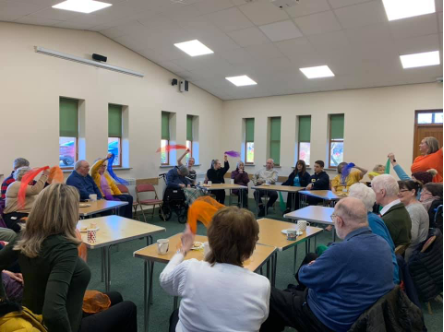
\includegraphics[width=.8\linewidth]{Images/ChapterFour/SilverlineCommunityRoomOne.png}
  \label{fig:communityRoomOne}
\end{subfigure}%
\begin{subfigure}{.5\textwidth}
  \centering
  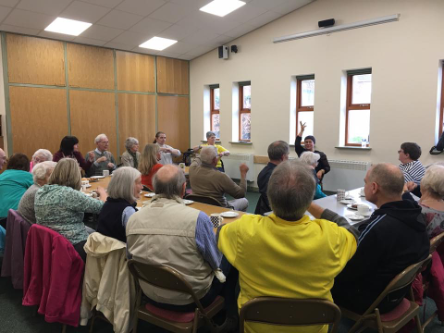
\includegraphics[width=.8\linewidth]{Images/ChapterFour/SilverlineMemoriesCommunityRoomTwo.png}
  \label{fig:communityRoomTwo}
\end{subfigure}
\caption{Silverline Memories community room (taken from Silverline Memories Facebook account)}
\label{fig:SilverlineCommunityRoom}
\end{figure}

For the first workshop, I wanted to find out what type of environments the members at Silverline Memories might want from a VR experience. Working alongside Dr Kellie Morrissey, we set out for Silverline Memories dementia café, and I felt nervous. I felt so out of place. Apart from my experience with my grandfather when I was a child, I had never really been around people with dementia. Kellie and I arrived at the dementia café a little earlier than Sandra. Sandra arrived later than us, with bags full of snacks and drinks for the members. As we approached the dementia café, we helped Sandra carry the bags into the  café (seen in figure \ref{fig:SilverlineCommunityRoom}). On the left side of the room was a kitchen area for volunteers to hand out tea, coffee and biscuits throughout the session. The area had an open plan layout that let volunteers and members help themselves freely. 

As I helped Sandra set up the room, I got my notebook out, a VR headset, a recorder, and consent/information sheets. As the first couple entered the café, Sandra and the other volunteers came over to them with open arms. They caught up, got them a drink and biscuits, and sat down. Sandra introduced the couple, Philip and Kate, who seemed happy to talk to us. They asked about the research and what we did. However, as I would find out later on, the initial few minutes of signing consent, reading information sheets and explaining the research could be uncomfortable for all those involved. At that moment, the situation went from an informal conversation into a formal study where two of us would be analysing and studying what was said. As we described the study, both were very happy to participate in the conversation about the types of VR experiences they would like to see. They were content with quotes being used as long as they were anonymised.

With VR being relatively new to the members, I began by introducing a simple VR experience which consisted of being able to navigate through a simple VR apartment space. The choice of an apartment VR experience was decided upon because of its neutral nature; it did not give any low or high expectations of what to expect with VR technology. After participants tried the headset, we spoke about the types of places they would like to see through it. I used printouts of images to further these conversations, such as images of libraries, museums, forests and beaches. During the first workshop, I spoke for an extended time with one couple, Thomas and Janet, where Janet was living with advanced dementia and struggled with verbal communication. Thomas told me about how he thought that Janet might like a VR environment that emphasised country music. From this, I decided to create a personalised VR experience based on her love for Shania Twain. I also set out to design and develop two environments for the dementia café. The first was a beach environment and the second was a park that took inspiration from a local park that participants had reminisced about in the workshop.

The workshop was my first experience working with people with dementia, but more importantly, the first time I would be seen as a `researcher'. I looked young and received sarcastic comments from the participants about my age and I did not know how to conduct myself in conversations with this new title. Each conversation felt like an interview, and I sensed a power imbalance. Kellie and I were the only ones walking around with the title of `researcher', who were here to interview and record participants. It was so unnatural to me, but why would it be natural? I do not start my conversations with friends or family with consent forms and placing an audio recorder on the table. Nevertheless, the methodologies I had read focused on the importance of researcher-participant relationships. For instance, \cite{mckillop2004make} highlight the importance of building relationships with people with dementia to make participants feel more comfortable in the study. The authors provide several strategies to improve engagement in interviews, such as talking about the person's life and what they have done today; being empathetic and caring in the interviews; and being flexible in the conversation to fit the participant's needs. At the time, this influenced how I approached my conversations with people with dementia where I would initially get to know them first and vice versa. From here, I would then continue with questions related to the design of the VR environments, while being open to what the participant wanted to talk about or interact with.

\subsection{Designing tailored VR environments}
\label{S1:VREnvrionments}

\begin{figure}
\centering
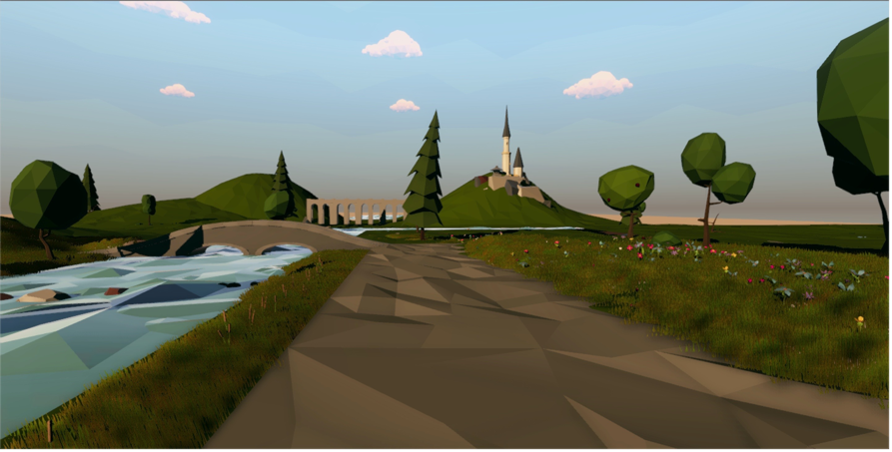
\includegraphics[width=.8\linewidth]{Images/ChapterFour/IrishCastlVR.png}
\caption{Park environment including an Irish castle}
\label{fig:IrishCastle}
\end{figure}

From the data collected from the first workshop, I created sketches based on individuals' ideas and desires. While I could not develop each participant's individual experience due to time constraints, some ideas were combined into one environment. For example, from my field notes, one participant asked me to \textit{`take [her] back to Ireland, to see the beautiful castles again’}. While I could not do that, I did create 3D designs of a traditional castle from Irish medieval architecture. We placed it in the park environment that many participants were interested in (see figure \ref{fig:IrishCastle}).

I created all three VR environments in the Unity game engine. I carefully planned the design of our environments in terms of the participant's field of view. I applied \citeauthor{alger_visual_2015}'s (\citeyear{alger_visual_2015}) concept of content zones (figure \ref{fig:ContentZone}) to reduce risks of sickness or disorientation and to improve the overall experience for the individuals. At the time, designing realistic VR experiences was limited to using 360-degree cameras. As I wanted to create experiences that might not be available, such as a 360-degree Shania Twain concert, the design of the environment was based on low-poly art that could not only can run on low-end hardware (a simple smartphone) but which also provided a very stylised and abstract view of the reality.

\begin{figure}[htp]
\centering
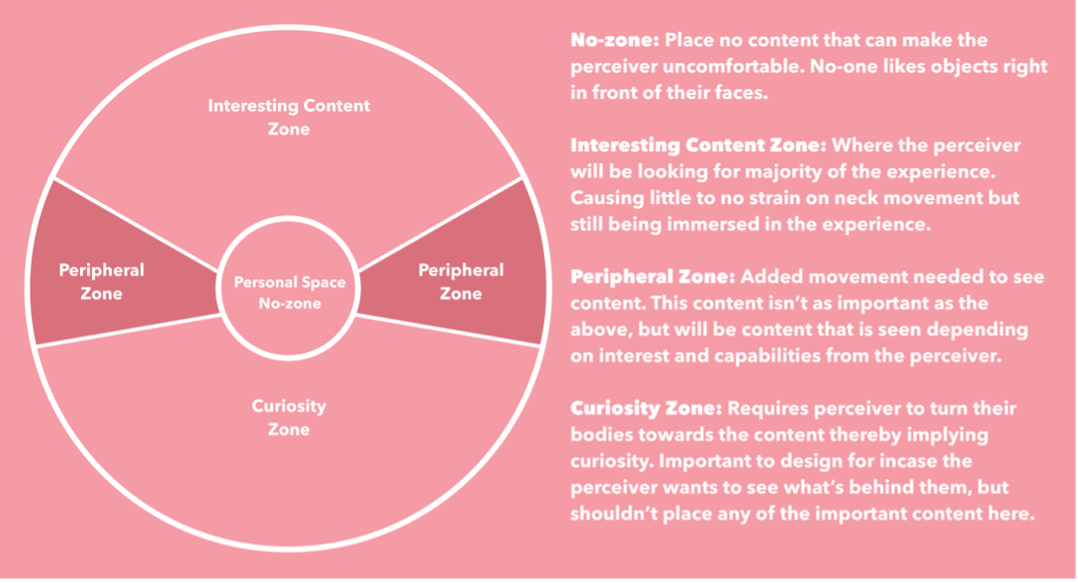
\includegraphics[width=.8\linewidth]{Images/ChapterFour/ContentZones.png}
\caption{Content zones in VR}
\label{fig:ContentZone}
\end{figure}

\subsection{Workshop two: ``Lighthouse, rocks, sand, sea, boat!''}
\label{StudyOne:WorkshopTwo}
In the second workshop, I returned to Silverline Memories to try out the different environments focused on the group at large: the beach with a horse running along the sand and a park based on a local park nearby, Jesmond Dene. Given that the charity won a lottery funding, the session was co-run with celebration activities, as a magician and a singer performed for the group. The celebrations put less pressure on me, as the entertainers kept the room occupied while I went around the room graadually and showed the VR environments to attendees. 

Several care partners and people with dementia tried the park and beach experiences and adored them. With encouragement from her daughter, Lucy, who was living with dementia, tried the beach experience and started listing what she could see — \textit{``lighthouse, rocks, sand, sea, boat!''} — as she rotated around and took control of the experience by focusing on the parts of the environment she found interesting. In this instance, Lucy was not a passive observer in the experience but, in fact, the focal point driving the experience. Lucy continued to talk about the experience to her daughter, which led to a shared experience for the two. In this way, the technology acted as a novel experience that provided an excuse or conduit for conversation - similar to `Ticket to Talk'. \cite{welsh_ticket_2018} discussed, in their design of Ticket to Talk, an app to provide conversational guidance in dementia, so that carefully designed technology may provide essential conduits for a social chat in dementia when social partners are unsure what to talk about. By tailoring the VR environments to the participants' interests, they would often comment on identifiable objects or reference memories associated with the beach or the park.

Lucy and her daughter were not the only pair who found the opportunity to share meaningful experiences. Many, if not all, participants expressed a wish to be able to share the same live VR experience as their partner or parent. When asked about this, participants indicated that meaningful shared experiences with their loved ones with dementia had changed recently or decreased in frequency. For example, Linda, whose husband Michael is living with dementia, mentioned that the couple no longer drive and had to use public transport. This meant that they could not visit favoured locations together, and so indicated that the VR park and beach could be used to supplement their recreational activities and allow them to experience a semblance of the sorts of activities that used to mean very much to them. Having the care partners experience the environment first allowed them to help to direct their loved ones around the environment by being able to probe specific interactions in the environment that the person with dementia might have missed. For instance, one care partner started asking questions about what they could see or if they saw the horse walk past on the beach. 

Near the end of the workshop, I sat down with Thomas and Janet to show them their personalised Shania Twain concert hall. With the current room getting quite loud, I asked the couple to sit down in the back room at the dementia café as a significant part of the experience was linked to the music itself. As I set the VR headset and passed it over to Janet, Thomas expressed some initial concerns about Janet having ‘the patience to hold the [headset] for a long time’. Thomas initially aided her in holding the VR headset:

\begin{quote}
\textit{Straight away [Janet] started to sing. She was singing to the tune and attempted to repeat the lyrics ... [and] changed her body language completely. It went from rather static, to movements that captured the tempo of the music. Janet held up her hands to try to hold the Google Cardboard as well, which indicated she did not want to stop the experience. [Afterwards], she seemed very happy and just from being around her, you could see her mood had changed completely.}    
\end{quote}

While Janet’s experience was heightened by her ability to recall the Shania Twain song, she got to experience it in a completely new way. Janet’s interests, body movement and interactions with others in the café changed after experiencing the concert hall. The bespoke design that placed Janet at its forefront provided her with the opportunity to control the experience by focusing on what interested her the most in the VR environment. Later, reflecting on the experience, Thomas mentioned that Janet \textit{``always sang and whistled. She can sing along to songs as long as she remembers the words. The aesthetic of the theatre was a great idea and gave a great sense of space''}.

\subsection{Reflections and outcomes}
\label{S1:ReflectionsOutcomes}
During the conducting of the study described above, I was able to have multiple conversations about dementia with my grandmother and understand her relationship with dementia. Through these conversations, I was able to connect to my grandfather, which I never thought I would have the chance to do. Listening to my grandmother's stories of looking after my grandfather painted a picture of a relationship with `ups and downs', with an overall positive perspective of dementia. However, only by spending more time at Silverline Memories did I gain a more in-depth understanding of the vastly different experiences people have with dementia. To conclude this section, I reflect on the following three areas, which arose for me in the course of the work and its write-up, and which led to future work for me:
\begin{itemize}
    \item Designing beyond reminiscence
    \item Challenges of designing technology
    \item Participant involvement in the design process
\end{itemize}

\subsubsection{Designing beyond reminiscence}
\label{ReminiscencevsMoment}
During the first workshop, participants mentioned particular locations that resonated with their childhood. For example, several participants who grew up in Newcastle described seeing Jesmond Dene Park or Whitley Bay Beach - both places being popular days out' places in the North East. During the conversations, participants would often describe structural details such as \textit{``I love the bridges over the lake''}, and stories of Whitley Bay lighthouse. Drawing on childhood memories mirrors the use of technology to support the collection of media such as photos, texts or other memorable artefacts from the person's past \citep{astell_stimulating_2010}. The media can then be used for conversation, reminiscence and interaction between the person with dementia and family care partners and care staff. As such, one of the key insights in this work was the wish for shared experiences and the potential for VR experiences to promote conversation. 

While prior work, including my own, has leveraged techniques such as reminiscence, I believe that this can limit the active participation of the person with dementia in these design processes in some instances. While reminiscence can provide opportunities for engagement \citep{gowans_designing_2004, yasuda_effectiveness_2009}, for some, it may merely cause non-engagement or frustration when not being able to remember a specific memory from their past \citep{lazar_critical_2017}. Furthermore, centring an activity around the stability of long-term memory can lead to distress and raised expectations for the person with dementia who may not connect with the activity meaningfully \citep{alm_communication_2007}. While Janet had a clear connection with the music of Shania Twain, which supported her overall enjoyment of the experience, the experience might have been uninteresting or frustrating to both Janet and Thomas if Janet had not recognised the music. Therefore, technology that requires the person to articulate past events may not be an appropriate activity to enhance emotional connection. Similarly, researchers might also ask how we could provide opportunities for people to interact with evocative immersive experiences with differing emotional valence. It could be that they are not necessarily ‘pleasant’ memories, but are not distressing, and are valid and important experiences with which it may be valuable to interact.

\subsubsection{Challenges of designing technology}
\label{S1:Robustness}
During the study, there was not enough time to develop a robust product that could stay with Silverline Memories. At the time, I knew that the three environments I made were very rough prototypes that were prone to breaking and very limited to working on my phone's hardware. Knowing the condition that these prototypes were in, I never thought they would be ready to be deployed and used without my assistance to set up and solve unexpected software crashes. \cite{hwang2020exploring} further discouraged leaving technology that might be in the prototype stages.

Additionally, \cite{hwang2020exploring} stressed the importance of care partners' and volunteers' training, configuring and supporting the person with dementia in using technology. Similarly, in this study, care partners demonstrated this role in encouraging the use of VR and asking questions about what the participant could see in the virtual environment. In this way, the leaving of technology requires more robust working products and upskilling of care partners or volunteers to know how to use the technology and support the learning process of accessing the VR apps. 

\subsubsection{Participant involvement in the design process}
\label{WhatExtentCo-design}
As described in the background literature and methodology, several researchers have innovated methodological approaches to support people with dementia to engage in the design and development of technology \citep{hendriks_challenges_2014, wallace_enabling_2012-1,lazar_critical_2017}. For this study, although I did not have sufficient time with all the members at Silverline Memories, I spent more time with Thomas and Janet to inform the building of the Shania Twain concert hall. In part, this was opportunistic from Sandra expressing interest on behalf of Thomas, who could see the potential value of VR for people with dementia. During the first workshop, Thomas and I spoke at length about the potential of VR and how Janet might use it. This led to talking about Janet's favourite songs and how Thomas curated YouTube playlists at home. By the end of the conversation, I had spoken to Thomas about building a concert hall around Janet's favourite musical experiences.

While we had generated an idea together for the VR environment based on Janet's interests, that was the extent to which people with dementia were involved in the generative process. In workshop two, people with dementia were involved in the evaluative stages to understand how they might use VR and the potential issues with current VR technology. Rather than the work being  a co-design approach, the process tended more towards a consultation of the types of interesting experiences people with dementia might need. Instead, a co-design process would have consisted of an extended time frame with different members of Silverline Memories. They would participate in several iterative stages of building VR environments by engaging with cultural probes, generative activities and prototyping. Additionally, given that Janet would rarely speak, Thomas spoke on her behalf and indicated the type of interests she might want. While this worked well in this instance, this raises several questions: To what extent can people with dementia contribute to design of technology? If they do so, are people with dementia acting as an equal partners in the discussion, or rather, engaging in a set of workshop activities that provide the opportunity to co-create? \citep{tsekleves2020engaging,lindsay_empathy_2012}

\section{Study two: Media capture of meaningful experiences}
\label{studyTwo}
A key finding from the work above was that VR environments provided a familiar experience that encouraged shared experiences with their loved ones. Motivated by the outcomes of the previous study, the following study worked closely with families living with dementia in order to create personalised media experiences. Taking account of the ecology of care of the person with dementia, which considers the person with dementia, friends, and family, care staff, the experiences I created in this study needed to be meaningful to the family and friends — not just the person with dementia. 

Working with Silverline Memories again, I carried out a Research Through Design (RTD) methodology. RTD is a way of doing research which is the practice of design used to address wicked problems \citep{zimmerman_research_2007}, which entail a sense of complexity, and which have no current solution. RTD seeks to address the problem within its current situation and is generally acknowledged to involve end users within the design process in order to result in the addressing of, and reflecting on, problems within the associated design space. The output of RTD is the creation of artefacts, digitally-mediated experiences, and systems, which are applied to new problems to create new knowledge \citep{gaver_what_2012,bardzell_documenting_2016}. The knowledge produced can only be elicited by the creation of these artefacts, which offer a novel and embodied method of knowledge production.

In this study, I worked with three families: two married couples, both with a wife living with dementia, and where the husbands had formed a close relationship through attending a support group. The third family was a family of four, where the father was living with dementia. The three families took part in day trips, which they co-planned, with data collection during these days providing insights into their shared social experiences. Workshops were also held  in order to personalise the experience of the media created during these days out. One output of RTD is the creation of artefacts, which resulted in the creation of `moment boxes' for the families to keep and use after the study. To respond to the reflections above, this study set out to tackle the reflections by:

\begin{itemize}
    \item \textbf{Designing beyond reminiscence}: Instead of relying on the person's abilities to recognise or articulate past events, this study orients experiences towards being in the moment and living a meaningful life with dementia.

    \item \textbf{Challenges of designing technology}: While this study focuses on building prototypes to explore the ways people with dementia might use technology, an output of this work is for the families to be provided with a VR headset and additional materials made post the end of the study. This is due to previous concerns about not leaving technology behind after a study is over.

    \item \textbf{Participant involvement in the design process}: In the first study, participants had little input on what would be created for the VR environments. This was primarily due to the short turnaround of the project. For this project, I worked with the families over numerous visits and co-designed days out to leverage the walking interview technique described in the methodology.
\end{itemize}

To begin conversations with families about participating in the project, I met the families at one of the Silverline Memories days out. I used this as an opportunity to get to know the families, explain the research and purpose. Sandra introduced the two married couples (Lauren, Michael, Sarah and John - also known at Silverline Memories as 'The Fabulous Four'), who seemed somewhat sceptical of participating. Initially, Michael jokingly would ask if I would be \textit{``spying on them''}, or how I \textit{``look awfully young to be a researcher''}. These jokes made me aware that I did not necessarily fit in with the group as I was not a member or a volunteer. At the time, I felt like I had to prove that I was invested in what they had to say, and I was not here just to collect data and then leave. 

Michael asked \textit{``why are you so interested in us?''} I told Michael stories about my Grandparent's relationship and how I wanted to know how technology could improve the quality of life for families with dementia. This led to Michael  opening up about the importance of relationships and friendship when Lauren was diagnosed with dementia:

\begin{quote}
\textit{``It's been a few years since Lauren was diagnosed with dementia, and Silverline Memories has been a lifeline for us. At first, I didn't know what to really do... We would just sit inside all day and Lauren would just look at the wall and not do anything. But then a friend of mine started to tell me to start going to these dementia activity days like Silverline, and that is where I met John and Sarah. Since then, it has been life-changing. We go on holidays, spend most of our weekdays together, and try to do as much as possible.''
}    
\end{quote}

It was apparent how meaningful the relationship was between the four. Their relationship was not just about depending on one another for support, but a genuine friendship and connection had formed. As we continued to talk and spent the day getting to know the couples, Michael and John both ended up being very keen on taking part in the research. I sat down with the four of them, and we planned out a day out at a National Trust park in Northumberland. I took their phone numbers, and we scheduled the rest of the day out over the phone.

\subsection{Day out with `The Fabulous Four'}
\label{DayOutOne}

\begin{figure}[htp]
\centering
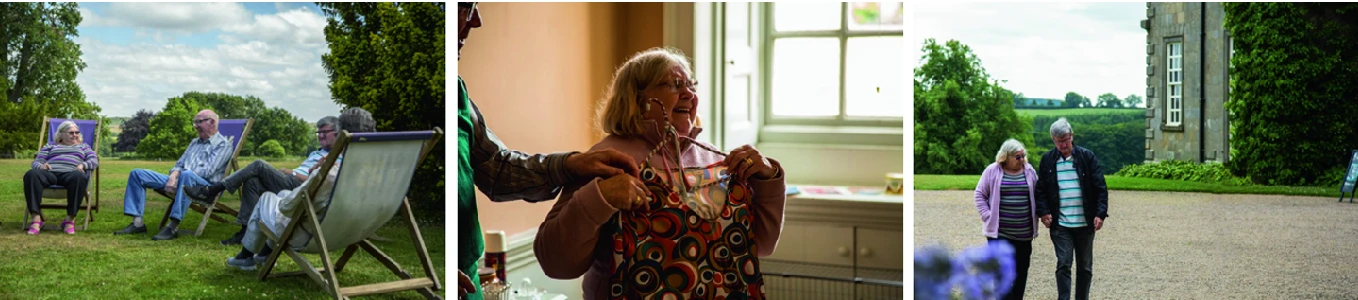
\includegraphics[width=1\linewidth]{Images/ChapterFour/FamilyDayOut.png}
\caption{The Fabulous Four day out}
\label{fig:DayOut}
\end{figure}

For the first day out, I went out on a day out with the fabulous four - John, Sarah, Lauren and Michael. The families decided on the National Trust Site in Northumberland as this was a place that Michael and Lauren had become fond of over the past decade. As travelling can cause discomfort to many, I hired the driver (Dave) from Silverline Memories, who not only gave comfort to the families as he was a familiar face, he acted as a tour guide. The family directed our day to capture moments they would like to experience again through personalised media. Our days out for each family followed a very similar pattern. On arrival of the desired location, families took charge of activities and route to take on foot while I accompanied the families. Activities included lunch, walking by the pier, engaging with the history of the place through museums and tourist guides, and conversations of getting to know one another and sharing our own stories within the group. As a family, they decided on the places and moments they wanted to capture through the 360-degree cameras and photographs. Throughout the day, our conversations followed a loosely-structured interview technique where we had a set of questions to address in our conversations, which we sought to address comfortably and naturally as possible through the six-hour long day out between the family and accompanying researchers.

The day started by sitting down at Michael's and Lauren's home, where the group suggested we meet. The pre-day-out conversation was relatively straightforward, reiterating the study and filling out consent forms. Once consent was filled in, Dave, the driver, drove the group to Wallington National Trust. Once at the site, I encouraged the family to decide where to walk through the day, including when they wanted to return home and if they wanted to sit down and have lunch or a rest. For capturing 360-degree videos and photography, the family would direct me around the day. For instance, John would suggest \textit{``Hey, can we go to the Chinese Pond and you could capture some videos of us walking through the place?''} Throughout the day, the interview process had an open-ended style and had the characteristics of a conversation rather than an interview. During the day, I would often lead the conversations by following up on the participant's comments about the day, or reacting to their nonverbal (i.e. picking up some bark on the floor through the forest).

\subsection{The families active role in the day out}
\label{ActiveRole}

Throughout the day out, interactions with the family seemed radically different from previous conversations. Having a continuous activity seemed to stimulate the sharing of knowledge between everyone involved. This section introduces three interactions with the couples, which shaped my understanding of walking interviews and allowed me to get to know the families.


\subsubsection{Taking lead}
\begin{quote}
\textit{   \textbf{Lauren}: ``You take note because I forget which way I come from, where I'm going to.''
}\end{quote}

\begin{quote}    
\textit{    \textbf{Researcher}: ``Don't worry. No problem. If we get lost, we'll get lost together. That's fine. It's so beautiful. You've been here quite a few times. Is that right?''
}    \end{quote}
    \begin{quote}    

\textit{    \textbf{Lauren}: ``Yes. Yes.''
}\end{quote}

Early on, Lauren expressed moments of anxiety regarding her orientation on the walk. Initially, she felt she could not take the lead and would rather depend on someone else on the day out instead. Gradually over the day, Lauren became confident in chatting about hobbies, interests, and directing me towards areas she found interesting such as showing me certain flowers she found pretty and miniature figurines found in the Wallington House.

Once Lauren gained confidence on the day-out, the walking interview format offered her to regulate our conversations by choosing different topics and having breaks together by sitting down at a nearby bench or slowing down. Lauren brought up topics relating to nature and the day out, which often led to Lauren asking me about what I do for work or wanting to look at the photos and videos that I had taken from the day. This starkly contrasted with my previous interactions with Lauren, where she would lightly acknowledge my questions and not lead the conversation any further. One reason for this, was that the walking interviews provided opportunities for one-to-one conversation away from Michael, her husband, who would typically speak on behalf of Lauren. In this way, walking interviews provided a safe space for one-to-one conversations where it allows Lauren to express her interests and even her own reality. As \cite{bartlett_citizenship_2014} writes, a sense of citizenship in dementia embraces the concept of choice and extends from person-centred and relational care. Including the individual's relations with others in the broader social-political landscape addresses influences regarding individual experiences and opportunities to grow and participate in life to the fullest extent possible. As such, the opportunity to walk alongside the participants made for a much more participatory, comfortable and supportive experience that suited the needs of the person with dementia.

\subsubsection{Carers sharing family stories}
Halfway through the day, the group stumbled across a set of folding chairs in the middle of the walled gardens. Sarah and Lauren suggested for us to sit down. As we did, Michael started to share a drinking and hunting tale from his past, which focuses on his own experiences, not those experiences solely with Lauren:

\begin{quote}
\textbf{Michael}:\textit{    ``We ended up in a little village called Farnworth. And in Farnworth there's a stream that runs through it. There is a road bridge, and underneath the road bridge, there is a deep place where you can get your horse in and you can wash all its legs off and get all of the mud off the bottom of it. Then . . . [a lady] went right under, which of course was hilarious to some of us who were still slightly uninhibited. But I can see the whole thing in my mind. It was just a fun day. It's all down to 150\% whiskey spirit.''
}\end{quote}

Over the day, I found myself getting many opportunities to get to know the care partners as much as the people with dementia. Traditionally studies often separate carers and people living with dementia as previous work expected different needs from one another. When care partners are designed for/with, technologies typically focus on duties of care with direction toward assistive technology \citep{bennett_assistive_2017, gibson2015everyday}. As Michael sees his wife within a social context, where she is more socially active and depends less on him, he feels like he is missing out. A common problem caused by close, intimate relationships is the overprotection and \textit{``doing too much''} for the person with dementia. This can lead to potentially depriving them as being agents who are able to initiate actions on their own self and can contribute to excess disability. For this reason, our VR experiences tailored for them combines 360-degree videos from their day out with a voice-over to explore the estate and history through the day out. Spending time with Michael and John, I started to understand the types of interests and desires they might want for the media experiences I eventually implemented into the moment boxes. In preserving this vividly-recalled memory through including it in the audio package received by the family, I sought to value the ecology of care around the person with dementia as well as the person themselves. In this way, the walking interviews offered insight into moments away from caring possibilities and dementia. Instead, Michael and John shared who they are rather than being defined by their roles. 

\subsubsection{Collaborative storytelling}
\label{CollabStorytelling}
In the house at Wallington National Trust, one room, in particular, caught Sarah and Lauren's attention. This room was filled with carefully modelled miniature figurines that both admired for a lengthy amount of time. During our time admiring these model houses and figurines, the interactions between the group could be seen as collaborative storytelling:
\begin{quote}
   \textit{\textbf{ Sarah}: ``Oh wow, look at how lovely these are!''
   *pointing at the miniature figurine set*}
\end{quote}

\begin{quote}
    \textit{\textbf{James}:  Imagine having one of these to play with when you were younger}
\end{quote}

\begin{quote}
\textit{    \textbf{Sarah}: ``Oh I know. It is incredible! Look at these little ones here'' *prompting me and Lauren to have a look*}

\end{quote}

\begin{quote}
\textit{    \textbf{Lauren}: ``Ah they're lovely aren't they''
}
\end{quote}

\begin{quote}
\textit{    \textbf{John}: ``You had something like that when younger Sarah didn't you?''
}
\end{quote}

\begin{quote}
\textit{    \textbf{Sarah}: ``Absolutely. its fantastic!''
}
\end{quote}

Continuing from the quote above, Sarah and John jointly shared the telling of Sarah's interests as a child. Although Sarah had difficulties in finding the exact words for describing her childhood miniature home, John supported the storytelling by structuring the story by asking Sarah questions he knew she could follow and answer. In this way, Sarah was able to keep her active role in telling her childhood stories.


\subsection{Day out with the Clark family - challenges with consent}
\label{ClarkFamily}
For the second day out, I invited the Clark family who expressed interest in going to Seahouses - a beach that held a place in the family's history. The family consists of Kate, her husband, Philip, who has advanced dementia, and their two daughters. On the day out, I met the group at their home and sat them all down to review the initial consent and information sheet. Philip, who was rarely verbal, and could no longer read or write, found it challenging to consent. Over a few minutes, his two daughters and Kate attempted to describe what we would be doing for the day out. This consisted of them describing it more enthusiastically than the more formal approach I took to the ethical description. However, while Philip retained a smile through his family describing the process to him, he never provided a verbal agreement to take part in the study at that very moment.

Regardless of not being able to record or take part in the research, I still took the family on the day out as the trip had been planned, and the sole purpose was to provide an enjoyable day out for the family. Throughout the day, Philip's interest in spending time with myself and his family became more apparent, and by the end of the evening, Philip started to take part in group conversations, tickle his daughters' necks, and say to his partner, \textit{``I love you''}. His family had rarely seen these acts from Philip over the past year. As with dementia, it is common for people to slip in and out of different abilities. At the time, I remember feeling frustrated that while he might verbally agree to the study, it was pointless as our day out was ending. Following the University's procedures, consent could only be signed at the start of the project. As \cite{dewing_participatory_2007} describe, traditional methods have often excluded the person with dementia by using a spouse or care partner to provide consent, and the consent process would never be revisited throughout the study. Instead, Dewing and others suggest a model where consent processes are a continuing consideration throughout the research project to provide informed flexibility and involvement from people with dementia \citep{dewing_participatory_2007,slaughter2007consent,mckeown_actively_2009}.

This model provides a strong understanding of the person with dementia to ensure the researcher can recognise the participants changing consent and assent over time. \cite{haraldsdottir2019relational} describe the process \textit{``highlights the ability for people to express choice and respond to experiential encounters and situations that remain long after cognitive decision making is reduced below the legal threshold for informed consent''} \citep[pg. 4]{haraldsdottir2019relational}. As such, the process of consent is highly flexible and situational. However, in contrast, when submitting the ethical procedures to the University Ethical Review board, it was relatively static and required to follow their set rules. While the ethical review board at the University is in place to protect participants and the research, If I could have sought support, advice, and had a more open collaboration through the ethical process, perhaps Philip's involvement in the research could have changed radically.

\subsection{Workshops}
\label{workshops}
Having captured a wide variety of data on the days out, I wanted to create ideas of how this data could be personalised and be used by the families. I invited families, designers, and dementia experts to individual family workshops to consolidate the personalisation and to store the created moments from their days out. In the workshop, I shared pictures and VR videos to give each participant a perspective of the day out and to see the digital moments that the families had co-created. The first workshop activity was for participants to create and share a salient memory from their past. The families were prompted to think of the context, the sensory stimulation, others involved in that memory, and then finally to share the memory with the group. The discussion then focused on how memories such as these could be translated into technological media in order to be able to relive or experience that memory in tandem with others. To structure this discussion of unfamiliar technological interactions, participants used an adapted version of Tiles IoT toolkit \citep{mora2017tiles}. Through the collection of the data from the days out, and the workshops, the following sections describe the ways the data influenced the design of the moment boxes.

\section{Developing a design rationale for the Moment boxes}
\label{DesignRationale}
This section drawing from the analysis seen in this paper, details the design rationale that informs the building of the moment boxes. 

In this section, I develop a design rationale for the moment boxes. This rationale pulls from the thematic analysis (further details of the findings seen here - \citep{hodge_exploring_2019}) 

\subsection{Tactile and tangible}
\label{DR:TactileTangible}
In \citeauthor{nolan_perceptions_2006}'s work on stigma, people living with dementia have reported a feeling of lack of confidence when going out and building new relationships \citep{nolan_perceptions_2006}. Through our conversations, Michael reflected on Lauren's social engagement at dementia coffee mornings, which she attends alone:

\begin{quote}
\textit{    ``I`m told that she participates, and that she is much better when I am not there than she is when I’m there . . . Very often she has got her hand on Kym’s walker (a friend), walking her down as though she is looking after her and helping her.''
}
\end{quote}

To allow for coherent continuation of Lauren’s sense of self, the moment boxes focused on ways to support and maintain a sense of self through creating activities that Lauren could use with others outside of her relationship with Michael. While this may seem like I am ignoring Michael’s needs, I am instead respecting the whole spectrum of relationships that individuals have within the ecology of care is important. Working from the insights, I note the following design needs:
\begin{itemize}
    \item The moment box requires an attractive design and to be easily transportable for the families to share with others.
    \item To have different physical objects that can be touched or played with while watching the media experiences between two or more people. 
\end{itemize}

\subsection{Providing choice}
\label{DR:ProvidingChoice}
From early on, I aimed to design the media experiences with not only the person living with dementia, but to include their family members and friends. Traditionally, previous work separates care partners and people with dementia's different needs from one another. When care partners are designed for/with, technologies typically have a focus on duties of care with direction towards assistive technology \citep{bennett_assistive_2017,bharucha2009intelligent,gibson2015everyday}. However, by spending time with the ecology of care, and focusing on memorable and pleasurable activities, the overall technology or activity tends to include a variety of interests and interactions from different stakeholders. With many carers reporting high levels of burnout and burden \citep{takai_experience_2009}, targeting carers as research participants worthy of digital interventions focusing on personhood (as much as we target those with dementia) means treating them with respect, and as whole persons, rather than defining them by their roles.

In the workshops, Michael wanted to share experiences that would place Lauren in memories that required to articulate past events as their history held significant importance to him. However, as I got to know Lauren through the study, it was clear that Lauren lacked recognition of memories. For this reason, the media experiences within the moment box need to provide the opportunity for care partners to express their experiences through recognition, and if their spouse chooses to do so, they can join the experience too. In response, the media experiences need to consider the following:
\begin{itemize}
    \item The experiences must consider the different interests of the family members as well as the person with dementia. 
    \item To provide opportunities that do not rely on recognition of past memories.
\end{itemize}

\subsection{Nurture caring relationships}
\label{CaringRelationships}
In the study, the participating families were aware that my intentions were to design media experiences not only for the person with dementia, but for family members too. For instance, while Sarah and John were interested in, and excited for, sharing experiences with the different forms of media, the couple focused more on the day out itself when talking to me in the workshop, rather than speaking very much about the technology itself.

From my observations, it was apparent that Lauren and Sarah had a supportive relationship where they always checked up on one another. In a conversation with Michael, he recalled their family holiday with Sarah and John, and Michael mentioned that Lauren and Sarah \textit{``walked up the seafront hand in hand all the time, chatting away. What they talk about, one never knows''}. In this way, I sought to create a set of videos and photos that are focused on their relationship solely - with audio extracts of their conversations placed over videos I captured throughout the day, including intimate moments between the two showing friendship and respect for one another, acknowledging the other's dementia and increased need for care. With this in mind, the moment box requires the following design needs:

\begin{itemize}
    \item Design multiple ways to interact with the different data the family curated on the days out.
    \item The moment box needs to consider the different relationships between the couples, i.e. Sarah and Lauren's' relationship.
\end{itemize}


\section{Moment boxes}
\label{MomentBoxes}

\begin{figure}[htp]
\centering
\includegraphics[width=.8\linewidth]{Images/ChapterFour/MomentBoxespng.png}
\caption{Moment box}
\label{fig:MomentBoxes}
\end{figure}

Based on the above, I created each family a moment box to support families to revisit their captured moments from the days out. In this section, I describe the individual components of the moment box that have been designed in response to the different interests and desires of the family members and the person with dementia. Each moment box came with an Oculus Go Virtual Reality headset, a personalised wooden picture box, and a bamboo wooden box filled with physical objects from the days out, or specific requests from the participants such as the dioramas. The moment boxes are split into the following: a) VR tour, b) bamboo box, and c) picture box.

\subsection{VR Tour}
\label{VRTour}

\begin{figure}[htp]
\centering
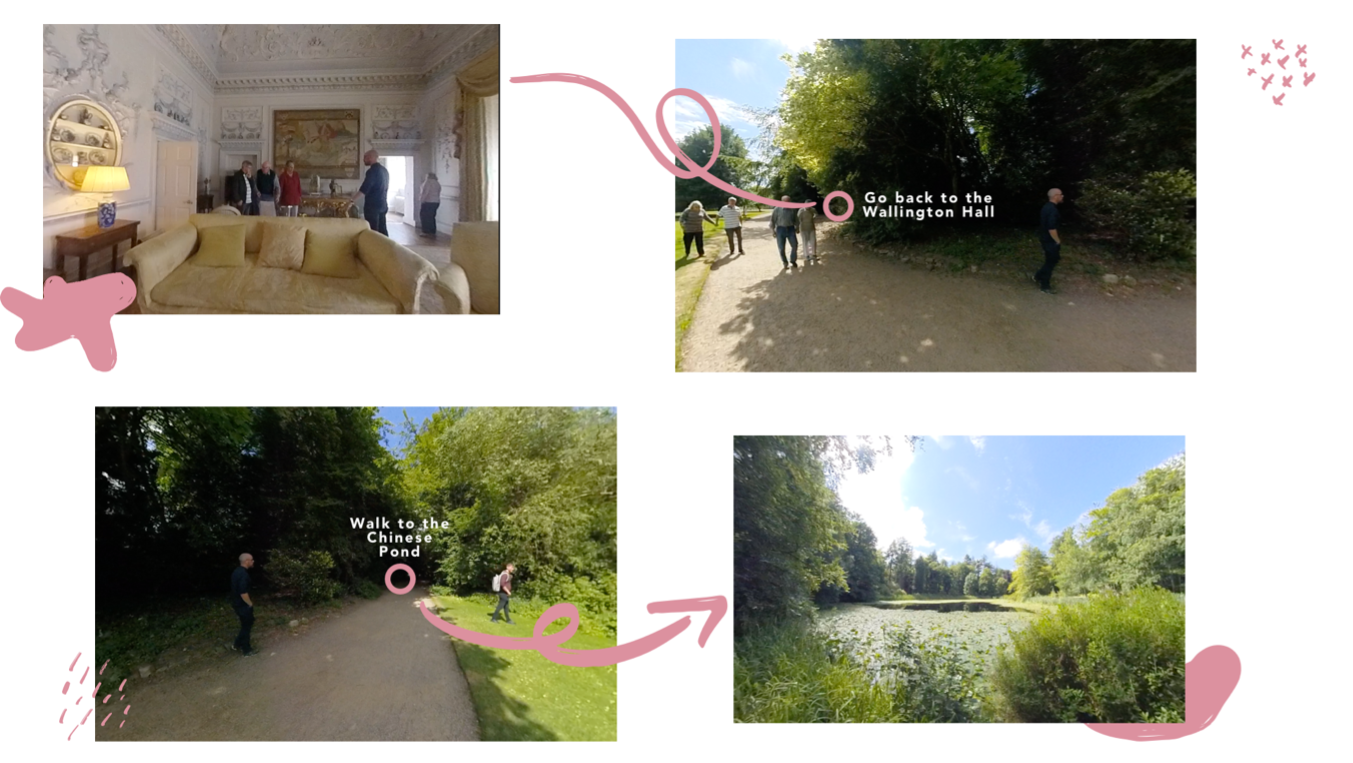
\includegraphics[width=.8\linewidth]{Images/ChapterFour/WalktrhoughOfWallington.png}
\caption{Walkthrough experience of Wallington Trust}
\label{fig:wallingtonTrust}
\end{figure}

Participants wanted to explore the day out through the captured 360-degree videos. To do this, I designed a ‘walkthrough’ experience where the user could navigate different areas of their day by clicking on pink circles on the video within the VR headset (see figure \ref{fig:wallingtonTrust}). For example, clicking ‘Walk to the Chinese Pond’ from the entrance video will take you to the Chinese Pond video. By capturing the footage with a 360-degree video, exploring the tour allows the user to freely choose what they want to focus on. For instance, in figure \ref{fig:capturedFootage}, the user using VR can either look towards their left to explore the flowers in the walled garden, or look to the right and follow the family walk through the park. This means that for Lauren, the moments are less about revisiting the past, and instead provide her freedom to explore the surroundings. 

\begin{figure}[htp]
\centering
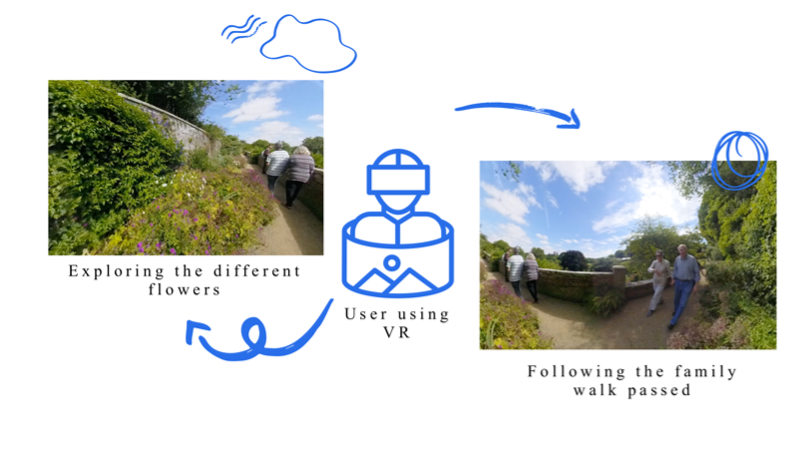
\includegraphics[width=.8\linewidth]{Images/ChapterFour/WaysToViewCapturedFootage.png}
\caption{Different ways to view the captured footage}
\label{fig:capturedFootage}
\end{figure}

\subsection{Bamboo Box}
\label{Bamboo box}

\begin{figure}[htp]
\centering
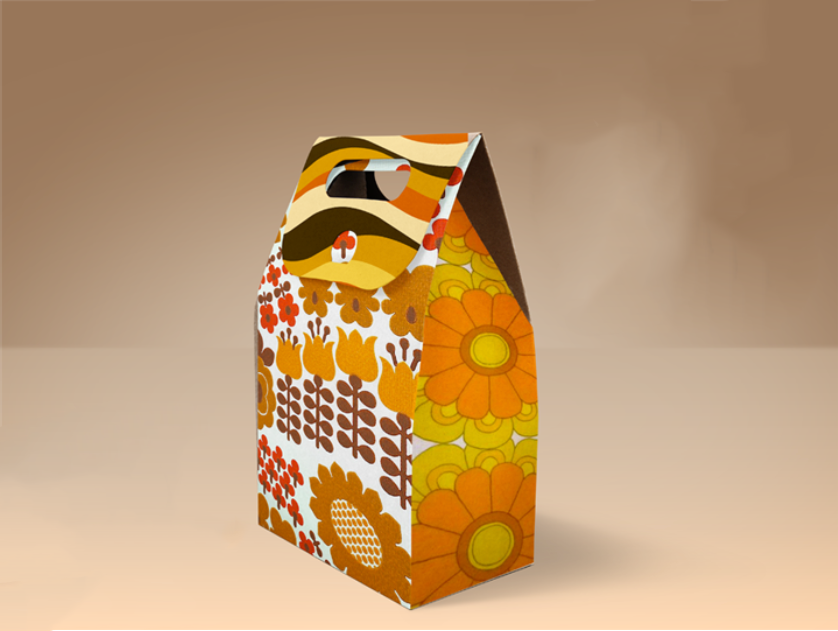
\includegraphics[width=.6\linewidth]{Images/ChapterFour/originalDesign.png}
\caption{Render of the original moment box with handle}
\label{fig:oldDesign}
\end{figure}
Family members described the types of material for the moment boxes. Through a couple of iterations and engagement with family members, bamboo was decided to be light and sturdy for the box. While this limited the customisability of the cardboard boxes, they remained sturdier and would last longer. In one of the workshops, Kate shared \textit{``Philip likes to pick at things or pull at corners of card. . . I think the boxes would have to be wooden or made out of something more solid so it can last longer''}. With more time, I could have created a more personalised box with a custom-made handle and lock on the sides to make the item more portable. Still, given the complexity and time it would take to create, I had to sacrifice particular design decisions (figure \ref{fig:oldDesign} shows an earlier design with a handle and lighter build). The bamboo box splits into two smaller boxes that consist of a) dioramas, b) storage for the QR code moments. I describe these below:

\subsubsection{Dioramas}
\label{Dioramas}

\begin{figure}[htp]
\centering
\begin{subfigure}{.5\textwidth}
  \centering
  \includegraphics[width=.8\linewidth]{Images/ChapterFour/Diorama1.png}
  \label{fig:DiroamaOne}
\end{subfigure}%
\begin{subfigure}{.5\textwidth}
  \centering
  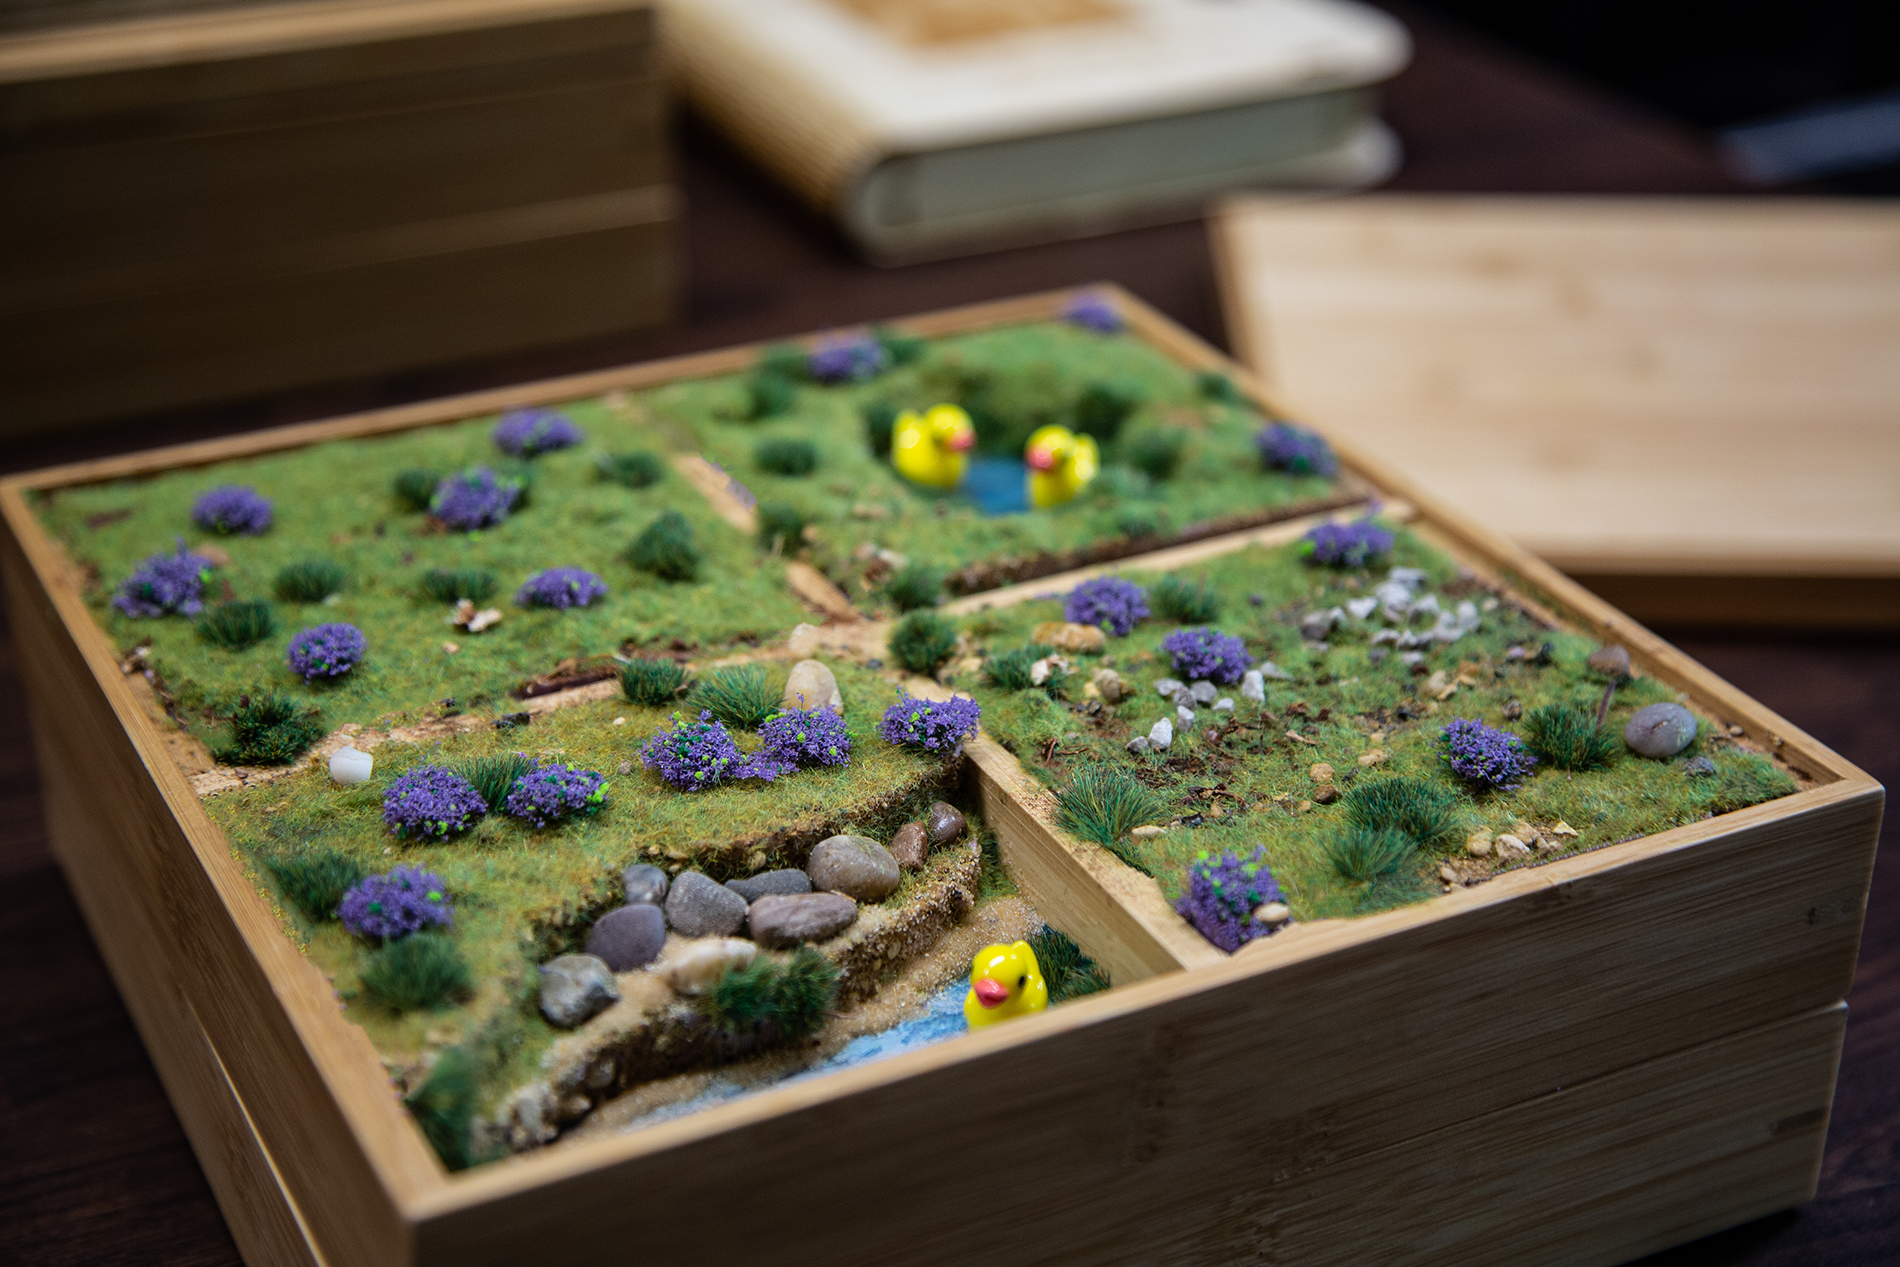
\includegraphics[width=.8\linewidth]{Images/ChapterFour/Diroama2.png}
  \label{fig:DiroamaTwo}
\end{subfigure}
\caption{Dioramas created for Lauren and Sarah}
\label{fig:Dioramas}
\end{figure}

Throughout getting to know the participants with dementia, they reported a range of interests in playful tangible objects that they could hold, feel and smell. For instance, Sarah would pull bark off the trees to play with as we walked through the forest. Further, as described earlier, Lauren and Sarah seemed fascinated by the miniature figurines and homes on their day out. With this in mind, the top tiered section of the moment box is a set of personalised dioramas. For each family, the dioramas are inspired by the days out. While the one on in figure \ref{fig:Dioramas} represents the Wallington National Trust Chinese Pond, they are designed in a way to remain abstract enough to be enjoyed by others. To make these dioramas, I first sketched a set of ideas based on the photos I had taken on the day out. Once I had chosen Chinese Pond, I bought a variety of materials such as miniature flowers, rocks, bark, and grass. From here, I built different sets out of Yoga matt material as this provided ease for layers.

\subsubsection{QR moments}
\label{QR-Code-Moments}

\begin{figure}[htp]
\centering
\begin{subfigure}{.5\textwidth}
  \centering
  \includegraphics[width=.8\linewidth]{Images/ChapterFour/InsideQRCode.jpg}
  \label{fig:insideQRBox}
\end{subfigure}%
\begin{subfigure}{.5\textwidth}
  \centering
  \includegraphics[width=.8\linewidth]{Images/ChapterFour/QRCode.jpg}
  \label{fig:QRCode}
\end{subfigure}
\caption{QR codes VR activity}
\label{fig:QRcodes}
\end{figure}
Lauren and Sarah described how they wanted to share some of the captured experiences with others at Silverline Memories. As the two of them had little interest in taking the headset with them, I provided a lightweight alternative that was east to use. In the bottom section of the bamboo box, is a set of QR codes that, once scanned, opens up a moment that the family captured on the day out. To provide steps to use the QR codes, the user places the QR code into the square (shown in figure \ref{fig:QRcodes}), and follows the steps on the side. I decided to laser cut the QR codes to give them a tactile feel where users could share them around without being easily damaged.

Kate and Philip's daughters mentioned they would like to capture their own 360-degree videos as they thought recording more moments \textit{``would be a lovely thing to do''}. To support the family, I designed tutorial guides, to create 360-degree videos for their family gatherings. Upon capturing the moments, the family can place their videos on YouTube and generate QR codes (see figure \ref{fig:QRCode-Captured}), which can be used similarly to the above but with postcards instead. While time spent with the family can increase Philip’s meaningful interactions with the family, a family archive of moments might provide Philip the opportunity to interact and experience familiar positive memories through hearing and seeing his much-loved family interact with one another.

\begin{figure}[htp]
\centering
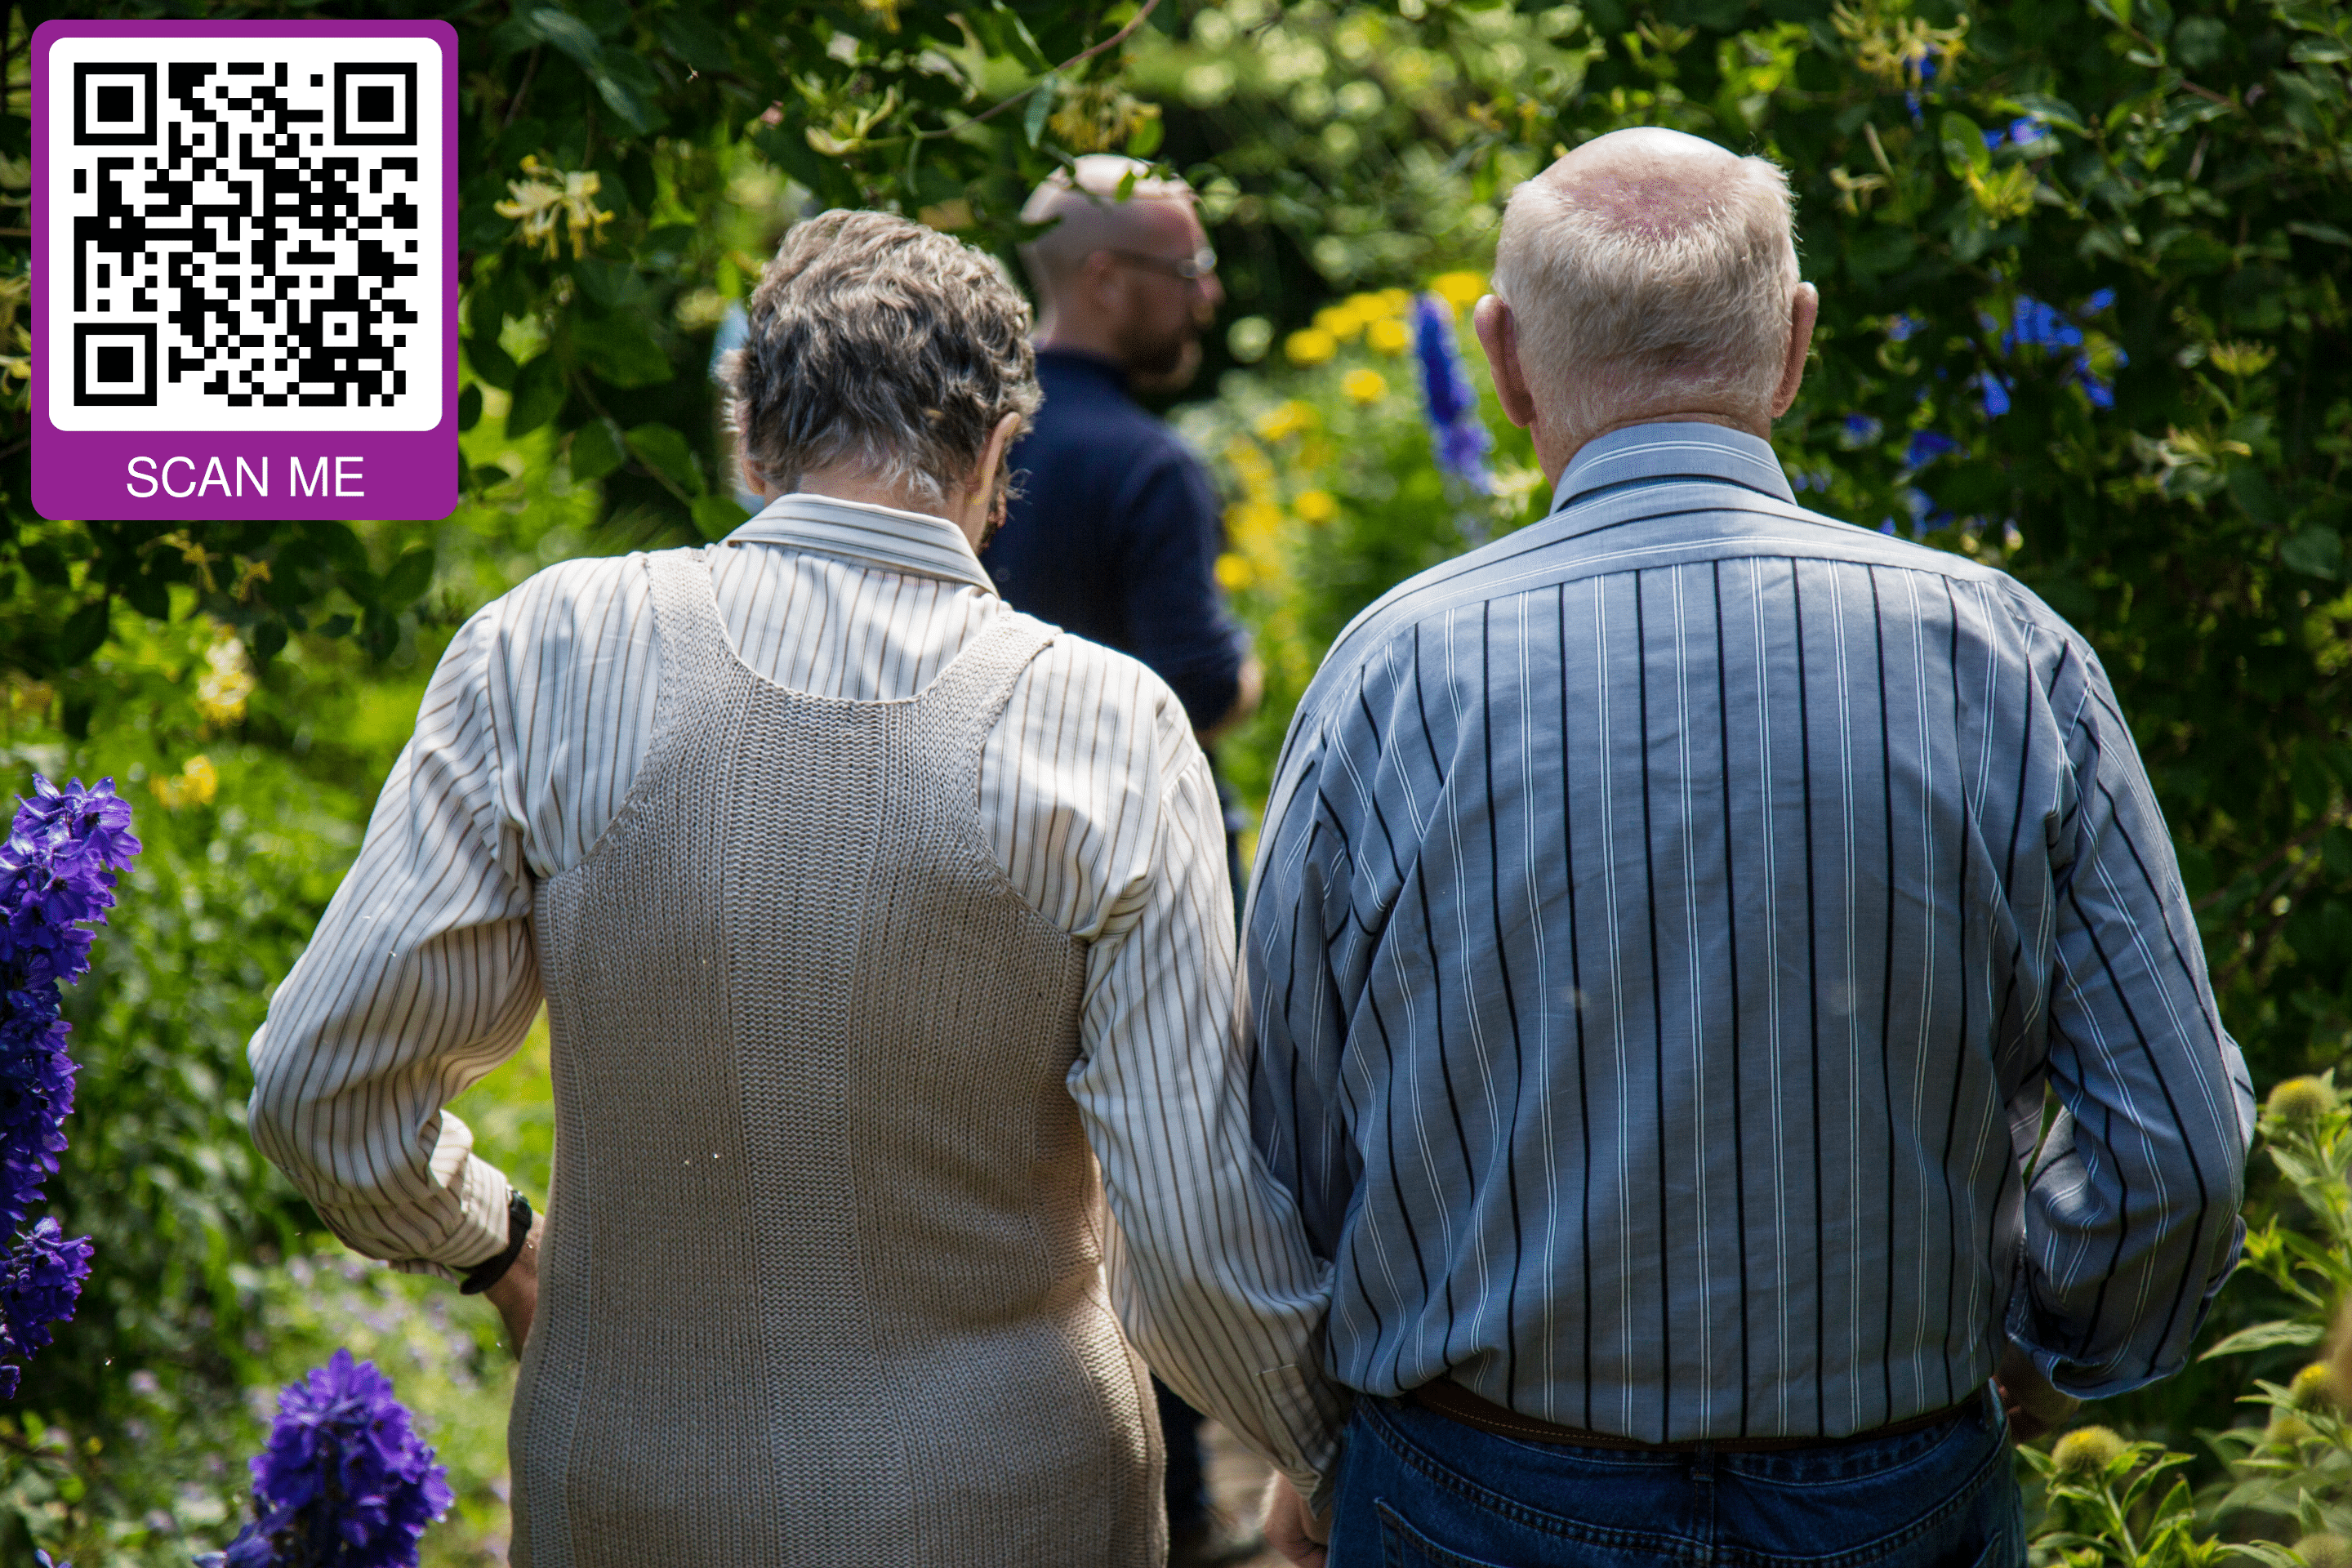
\includegraphics[width=.6\linewidth]{Images/ChapterFour/QRScanPhoto.png}
\caption{Add QR code to family captured moments}
\label{fig:QRCode-Captured}
\end{figure}

\subsection{Picture box}
\label{PictureBox}

\begin{figure}[htp]
\centering
\begin{subfigure}{.5\textwidth}
  \centering
  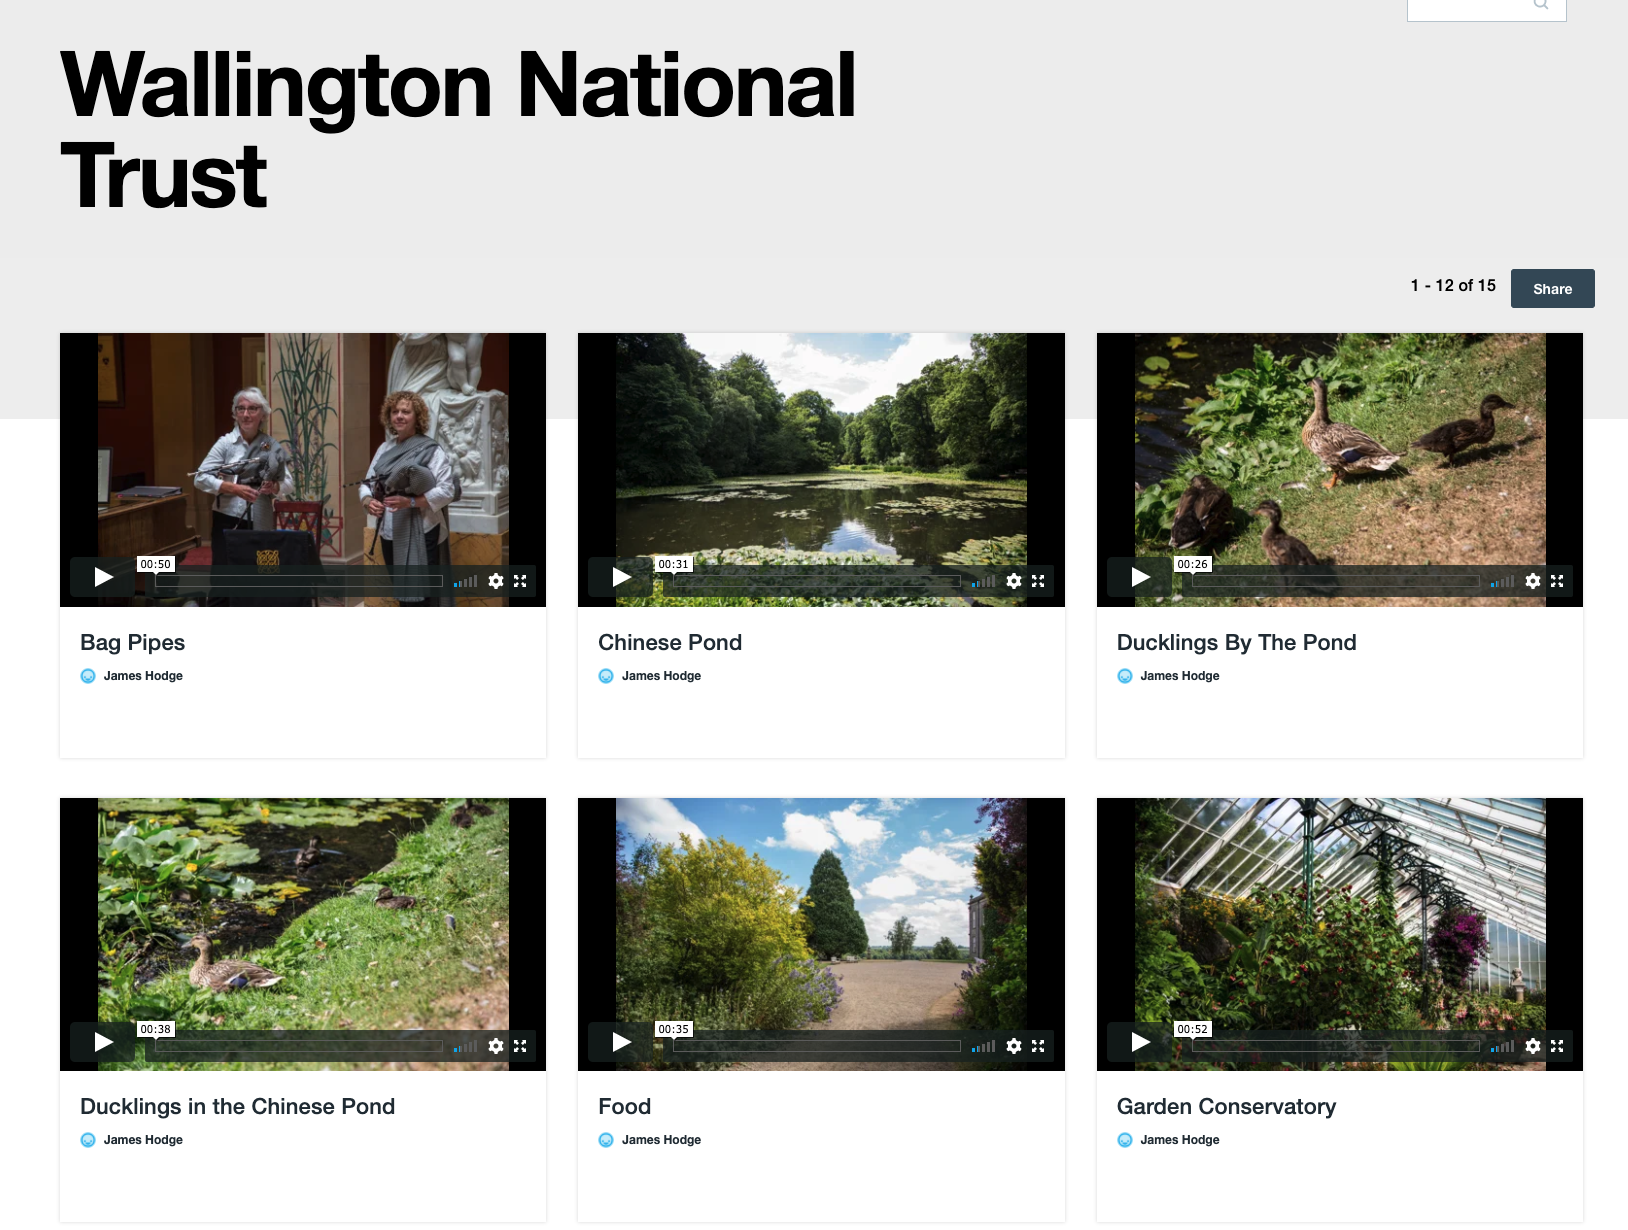
\includegraphics[width=.8\linewidth]{Images/ChapterFour/VimeoWebsite.png}
  \caption{Online archive on Vimeo}
  \label{fig:onlineArchive}
\end{subfigure}%
\begin{subfigure}{.5\textwidth}
  \centering
  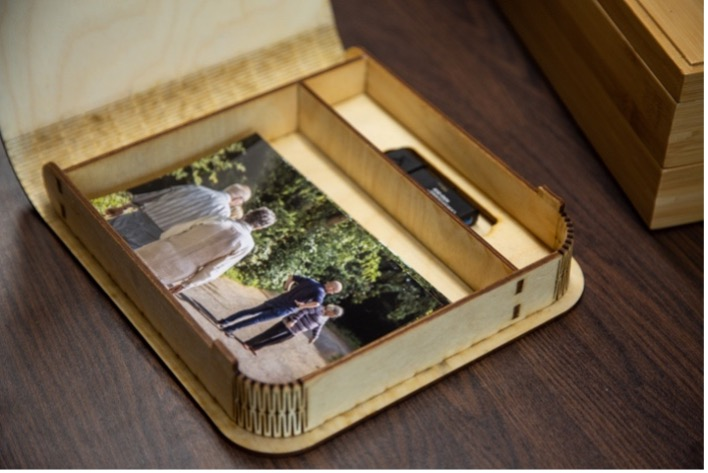
\includegraphics[width=.8\linewidth]{Images/ChapterFour/InsidePhotoAlbum.jpg}
  \caption{Album box with USB Stick}
  \label{fig:AlbumBox}
\end{subfigure}
\caption{Optional ways to access bespoke moments}
\label{fig:OptionalMoments}
\end{figure}

From the days out, all participants expressed an interest in the photos I was taking and expressed how lovely they looked. To ensure that the pictures wouldn't be put away in a drawer to be forgotten, I designed an album box to contain the images and a USB drive with all the data collected from the days out and workshops. The data was theirs to keep, and if they ever needed to print out multiples of the images, or use the videos and audio for other reasons, they had the data to do so. Additionally, through Vimeo, I curated a showcase with an archive of all the videos taken from the days out (see figure \ref{fig:AlbumBox}). In the boxes, I printed out multiple small cards that families could share with others with a bit.ly link for others to watch the videos. 

\section{Reflections and outcomes}
\label{S2:Reflection}
Over these two studies, the work has indicated the challenges and opportunities for involving the different needs of family, friends, and the person with dementia. As the work moves towards appreciating the importance of being in the moment in dementia care, it became apparent that the initial starting point of using virtual reality was not the critical part of the research. This chapter resonates with prior research around people with dementia can still experience meaningful interactions, relationships, and activities at almost all stages of the condition \citep{kitwood1997dementia}. But with over-protection, stigmatisation, and emphasising on people’s lack of ability, many believe that people living with dementia are poor at social contact, which can then prohibit many from interacting with people with dementia \citep{christine_bryden_dancing_2005, riley_anxiety_2014}. In this section, I reflect on the three areas I set out to tackle at the start of the study.

\subsection{Designing beyond reminiscence}
\label{beyond-reminiscence}
In the second study, it was clear that attempting to refer back to older memories may cause frustration or confusion. Michael describes that sometimes he struggles to orient Lauren to reality, creating new experiences of grief when she is told, time and again, that her mother has passed away. Orienting the person with dementia towards the `right' reality has very little effect; if the dementia is sufficiently progressed, the person will simply forget this reorientation again. It is also considered to be poor practice \citep{cipriani_understanding_2014}. Dana Walrath's graphic novel Aliceheimer's, about her relationship with her mother, Alice, who has Alzheimer's, conveys accepting her mother's reality and often going along with Alice's reality:

\begin{quote}
\textit{"[the graphics novel], shows how we treated Alice's hallucinations and disorientation as a special power. Instead of fighting about what was really there or where each of us was, we let her ability to travel through space and time peaceably account for our distinct realities. This made it possible for me to read the symbols buried in her travels. As I created the art, I used symbols such as cut text form Lewis Carroll's Alice in Wonderland to make Alice's bathrobe, her favorite garment, to convey our magical approach to living with dementia" \citep{walrath2021aliceheimer,walrath2017end}}
\end{quote}

It is imperative to remember that a sense of self can come from more than just our ability to recall and recount memories. Working with people with dementia sensitively should push us to reflect on the structural challenges of understanding the reality of the person with dementia and designing for this often `dreamlike' state, depending on the stage of dementia \citep{bryden_before_2015}. Researchers should consider what it means to design media experiences for realities that may eclipse each other briefly rather than conflict with each other entirely. In a similar vein,  although in the study, I indicated how outside activities can be captured via media, I must stress that this is no substitute for going outside, or for care homes to replace gardening or nature walks with virtual realities of the same. Actually engaging in such activities has multiple psychological and physiological benefits \citep{gilliard_transforming_2011} — researchers should instead begin to think about how both activities can overlap and eclipse each other: for instance, participants could collect rocks from beach walks. Late, these could be fitted with RFID tags which, when touched or otherwise triggered, play back captured audio or videos.

\subsection{Challenges of designing technology}
\label{robust-tech}
When reflecting on the two studies, a critical distinction between the two is that study two provides the participants with the physical moment boxes to keep and use. While building the moment boxes took considerably longer than I anticipated, due to other PhD commitments such as conferences, paper writing, and presentations, I delivered the moment boxes to the families about six months after the data collection. At first, I tried to contact Kate and Philip, but had no luck in reaching out to them. Later through Silverline Memories, I found out they were going through some family problems. For the other family, I met them at Michael's house, where I sat them down and walked through the moment boxes.

I placed the boxes between couples – one for Michael and Lauren and another for Sarah and John. They took the tops off the moment boxes, which revealed the personalised dioramas. Both said they \textit{``love it''} and started to feel and play with the grass and ducks in the ponds. After showing the album box with the photos from the days out, Michael asked, \textit{``What about the VR? I'm dying to try it''}. I took the VR headsets out, and we discussed how to set them up and what the headset can do. John and Michael grabbed the headsets and placed them on together. As I directed them through the range of settings, they both started to talk and interact with one another as they explored the 360 experiences:

\begin{quote}
\textit{    \textbf{John:} ``Here..Michael, are you seeing this? I see the house and you chatting to our James.'' *laughter*
}
\end{quote}
\begin{quote}
\textit{    \textbf{Michael}: ``Hang on a sec. . . I'm at the Ponds. Come to the ponds. How does he do that James?''
}
\end{quote}
\begin{quote}
\textit{    \textbf{James}: ``Flick the top button of the controller in your hand and you'll start moving between the different 360 videos.''
}
\end{quote}
\begin{quote}
\textit{   \textbf{ John}: ``Ah this is canny James.''
}
\end{quote}
\begin{quote}
\textit{    \textbf{Michael}: ``Look at the little chickens.''}
\end{quote}
At the time, Sarah and Lauren didn't seem interested in the headsets. They were laughing at John and Michael's interactions alongside me. Michael and John had expressed earlier in the study that they had iPad's and would like to see the experiences using non-VR technology. I introduced the QR code activity and described it to the four. As Lauren and Sarah grabbed a random QR code, looking slightly unsure of what would happen, Michael and John scanned the code on their tablets and rotated their iPad to move the 360 video.

A couple of weeks later, I had a brief call with John and Michael about their interactions with the moment boxes. Sarah and Lauren had spent very little time experiencing any of the VR experiences but would sometimes sit down and play with the dioramas, the photos, and the laser-cut QR codes. Sarah found the burnt lines in the plywood to create the QR code interesting to feel and hold. Michael and John felt guilty that what I had made wasn't being used as much. As we discussed that this would be the end of the study, both thanked me for all the work and Michael said, \textit{``if you are ever doing this again. . . we'd be more than happy to go on another day out''}.

While the families were thankful, it sounded that the VR headsets were not really used by the families. If anything, the use of VR was driven by myself and Sandra at Silverline Memories. Instead, John mentioned how he and Sarah loved \textit{``being the centre of attention on the day out, and its been so lovely to get to know you James''}. In a way, the building of relationships between myself and the families was held at a higher significance than the moment boxes.

Throughout this process, learning how to tailor the moment boxes and virtual reality environments has been a long and complex process. It has taken a long time to build relationships with participants who would then be willing to share their experiences. Not only that, in many cases, I had to learn new ways to adopt the methodologies better to suit the needs of the person with dementia. All the lessons I have learned to work in such a complex space were far from being covered in the Computer Science course. While computer science may not be the most appropriate place to learn about sensitive topics like dementia, opportunities to grow these skillsets in the early stages of developer and designer careers could be developed through participating in public events such as hackathons, blogs or online presentations.

Similarly, \cite{hendriks_valuing_2018} has considered novel approaches to undergraduate education to provide budding designers and developers with the skillset to make more sensitive design choices. In dementia and HCI, this has invited students to collaborate in co-design methods with care home residents by developing life story work \citep{mckeown2015you} and storytelling projects \citep{hyden2013storytelling}. However, while opportunities to work in more non-traditional settings such as care homes may be possible through university classes, these are often limited to a small, selected group of students or courses focusing on healthcare and psychology \citep{kinnunen_understanding_2018}, meaning those who are taught technical or design disciplines through university miss out on opportunities to gain experience with the vulnerable populations that they may end up building for. 

\subsection{Participant involvement in the design process}
\label{extent-co-design}

\cite{sanders2008co} states that end-users \textit{``plays a large role in knowledge development, idea generation and concept development''} and that users require the appropriate tools to express themselves and convey that they are the experts of their experiences \citep{visser2005contextmapping}. However, as described in the methodology chapter, many commonly used participatory tools and approaches are not always appropriate for people with dementia. For instance, in the first study, Janet did not have many opportunities to share interests and desires. Instead, her care partner, John, provided insights into Janet's music interests and the potential use cases for VR for her. In contrast, by designing days out with families in study two, I was able to get to know the participants with dementia through other means that moved beyond verbal expressions. \cite{hyden2013storytelling} argues that embodied movement can go beyond verbal expression and is an interactive process to participate in storytelling. Further, participants had control over pace, direction and topics on the days out. In this way, walking around a location puts less strain on verbal communication than the expectation to participate that people with dementia might feel in a sit-down interview or workshop. 

However, despite the participant's involvement in co-design the days-out, the extent to which participation can be described as co-design requires further consideration. From conducting these studies, they several challenges that question the abilities of people with dementia to contribute meaningfully to the co-design process. First, keeping participants anonymous is standard ethical practice when working in sensitive settings. However, doing so challenges the potential for people with dementia to share ownership and agency over publication and knowledge making. In study two, Philip's participation was complicated because he could not consent in the manner the university's ethical review board set out. It was evident within these two studies that participant involvement in design is central to designing sensitive and meaningful experiences. 

Second, as \cite{suijkerbuijk_active_2019} describes in her literature review on involving advanced stages of dementia in the design of assistive technology, the contribution that people with dementia have to the different phases of technology development varies. \cite{unbehaun_facilitating_2018} co-designed a set exergames that only involved caregivers and other stakeholders in the pre-design phase. Both of the studies in this chapter focus on the generative phase of design, where new ideas are constructed by performing participatory activities. In hindsight, inviting people with dementia to the pre-design phase may have provided insights into the different type of technologies they might want to use instead of VR. While prior work does suggest the difficulties in promoting the voices of people with dementia in the pre-design phase, future work should consider how to create tools that promote conversation between designers and people with dementia in this stage. By inviting people with dementia at the early stages, we can ensure co-design processes and studies are rooted in participant-led agendas and provide a more ethical research impact.


\section{Summary}
\label{C4:Summary}
In this chapter, I provide a reflective account of two studies where I worked closely with people with dementia and their family members. The focus of the chapter is to shine a light on the implications of designing participatory activities within this space. Through these studies, I reflect on recognising the role of the researcher as essential in building and maintaining relationships, and as a means of conducting engaged and impactful research. However, as I highlight towards the end, this has required working closely with people with dementia to engage in open and exploratory design responses to their lived experiences which needed long-term upskilling and education within HCI and dementia. Coming from a Computer Science background, I missed many opportunities to gain experience in social settings that I might be building for as a developer or designer. Ensuring I respected and involved people with dementia in varying ways throughout the studies required a longer-term commitment to get to know Silverline Memories, conduct the studies and learn about participatory methodologies simultaneously. However, this is not always possible in real-world design situations where research and design is done at a quick and agile pace. In response, the following chapter examines how students, developers and designers approach such a complex topic with little to no training. 

\begin{figure}[htp]
\centering
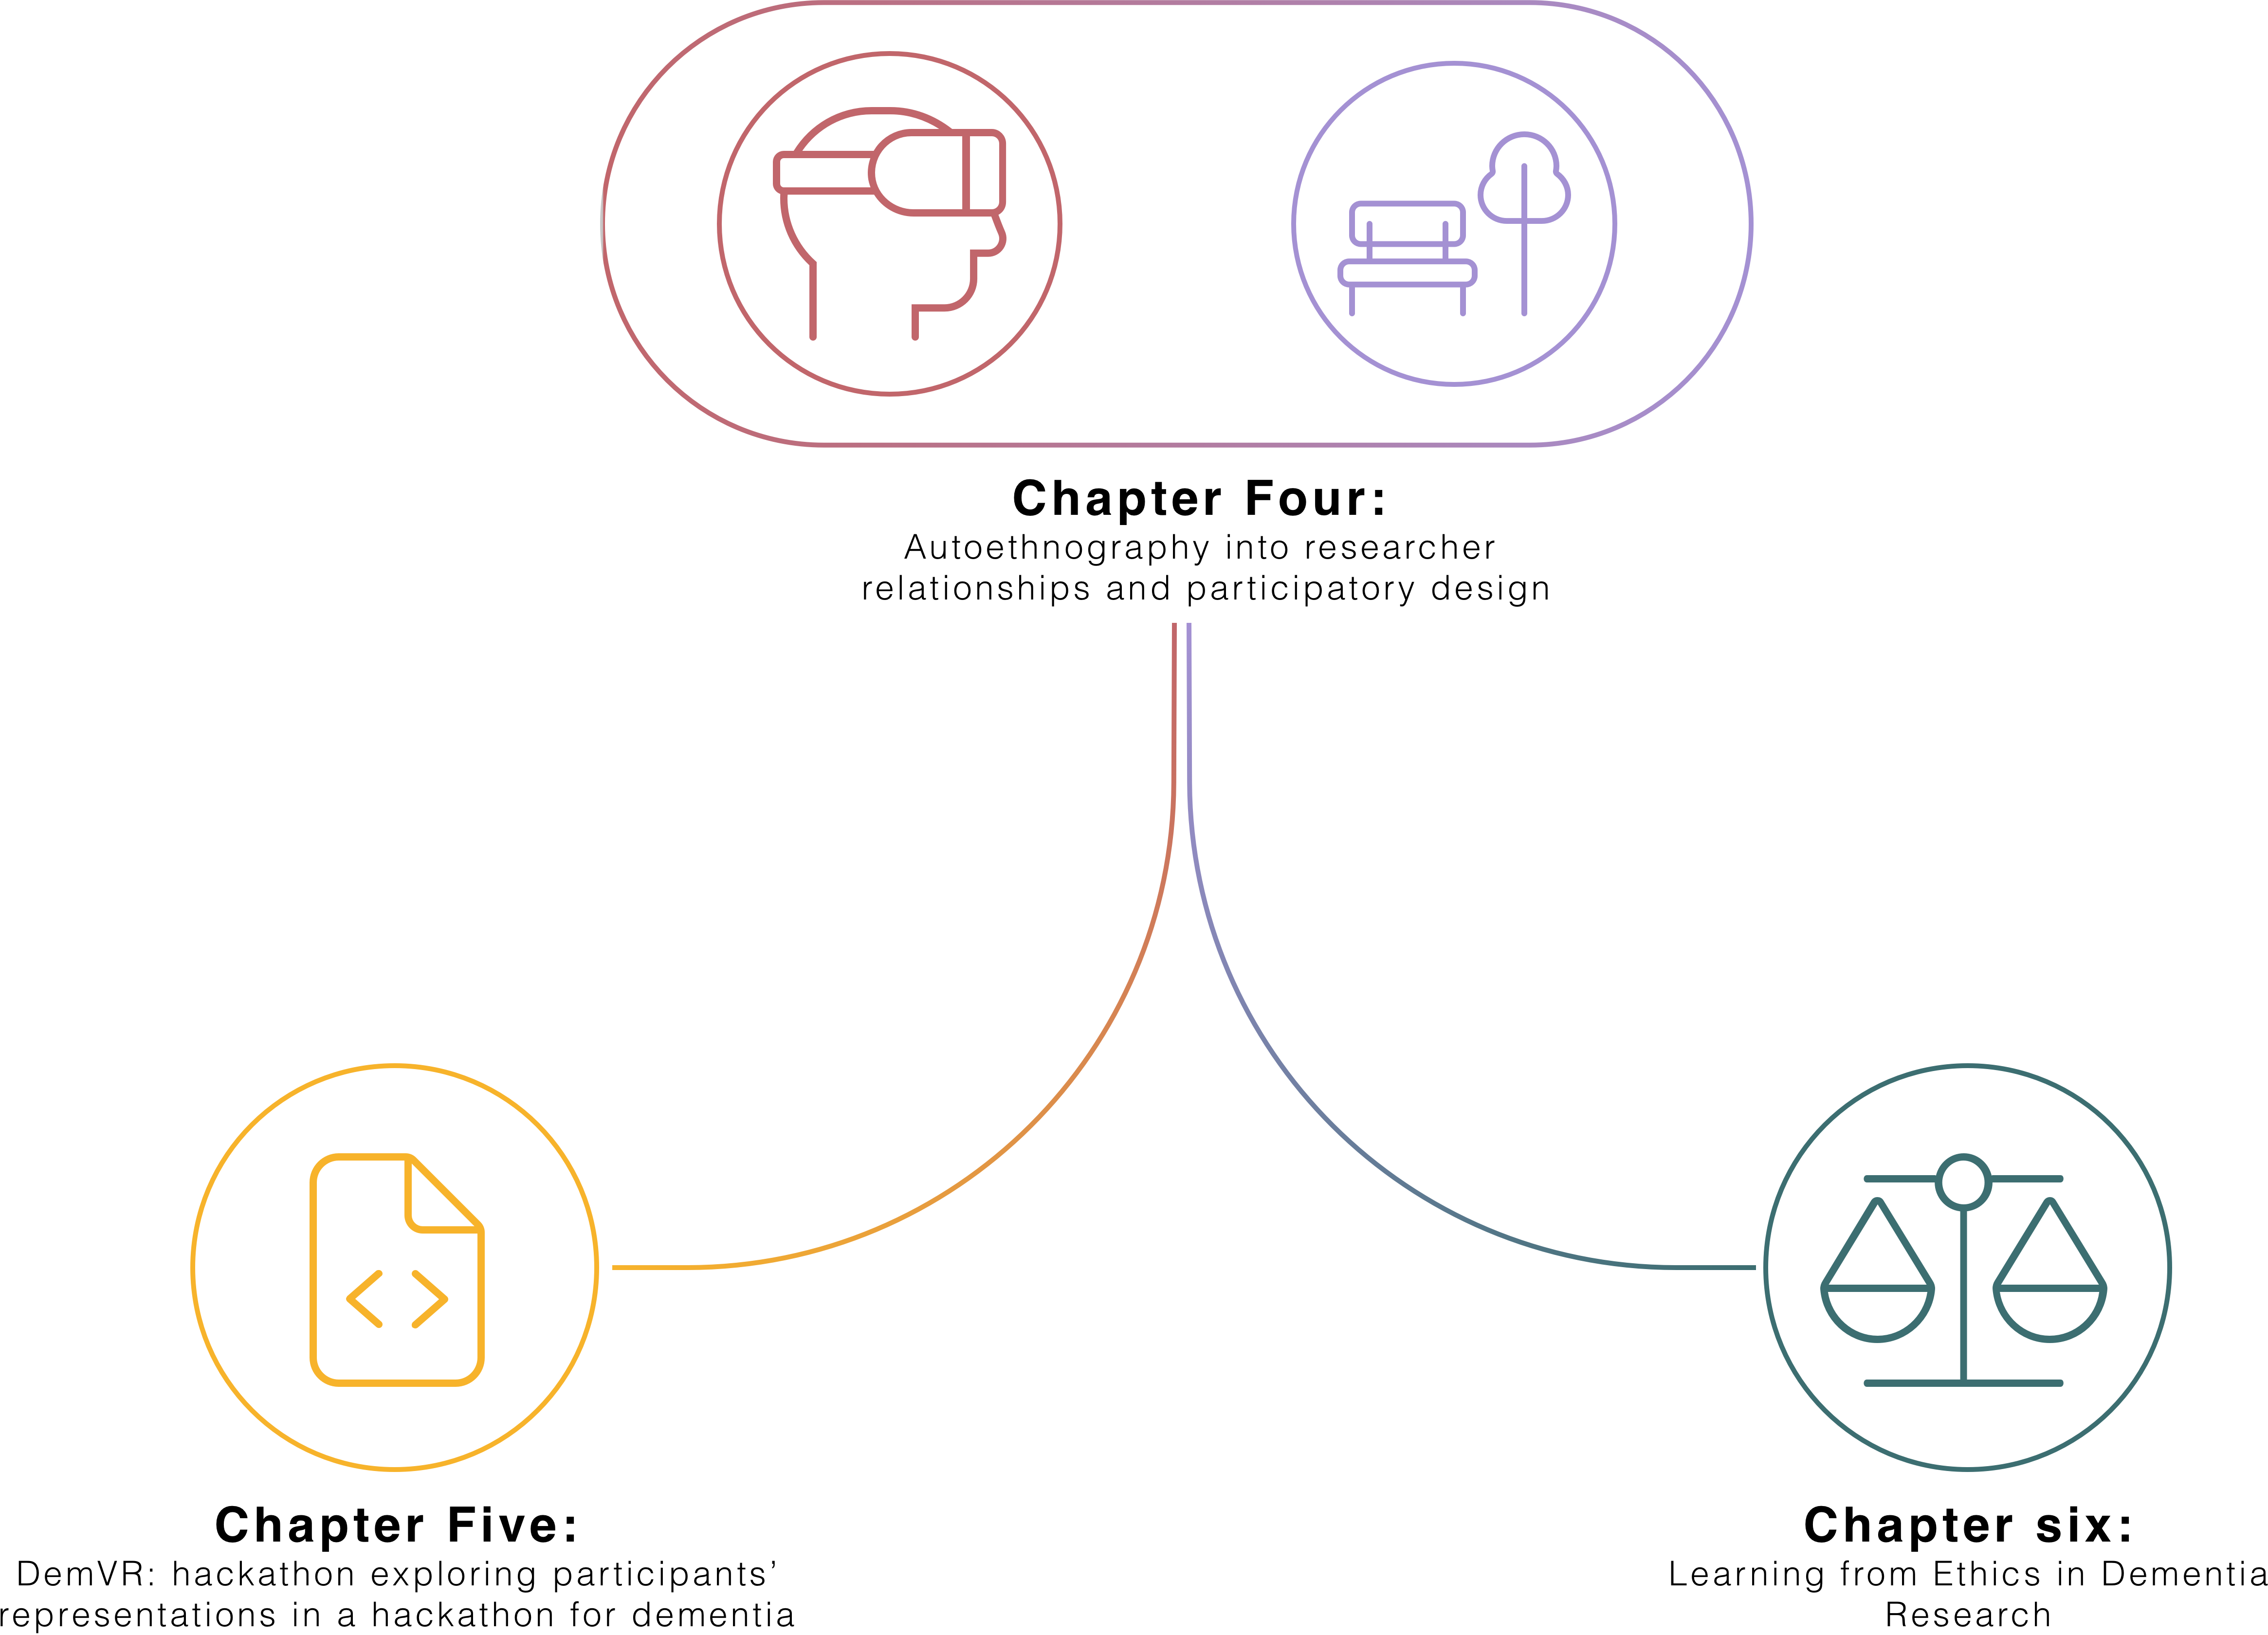
\includegraphics[width=0.6\linewidth]{Images/Thesis_Narrative/Narrative_ChapterFour.png}
\caption{Subsequent chapters}
\label{fig:ChapterFour_FutureStudies}
\end{figure}

Additionally, the research extends from person-centred approaches, which rely on relational processes as the basis of design. Through co-designing days-out and tailoring VR and media experiences with families with dementia, these studies provide insights into ways to treat the person with dementia as an individual; working within ecologies of care; and acknowledging that dementia is a complex experience that often also includes social complexity, ageing and multi-morbidities, which require attuning to in design and research responses. As such, this chapter also raises numerous ethical complexities such as consent, relationships and ownership in the co-design process. In response to the lessons learned, the following two chapters examine (see figure \ref{fig:ChapterFour_FutureStudies}): a) designers'/developers' shifting sensitivities about dementia in a hackathon aimed to provide a space for upskilling attendees on HCI and dementia, and b) the types of ethical concerns HCI researchers face in the dementia context.






